\documentclass[aspectratio=169,10pt]{beamer}
\usetheme{Madrid}
\usecolortheme{seahorse}
\setbeamertemplate{footline}[frame number]

\usepackage[utf8]{inputenc}
\usepackage{amsmath,amssymb,amsthm}
\usepackage{graphicx}
\usepackage{listings}
\usepackage{xcolor}
\usepackage{tikz}
\usetikzlibrary{arrows.meta,positioning,calc}

\graphicspath{{figures/}}

\lstset{
  basicstyle=\ttfamily\scriptsize,
  numbers=left,
  frame=single,
  backgroundcolor=\color{gray!7},
  keywordstyle=\color{blue}\bfseries,
  commentstyle=\color{green!50!black}\itshape,
  stringstyle=\color{red!60!black},
  breaklines=true,
  showstringspaces=false,
  language=Python
}

\newcommand{\B}{\mathbb{B}}
\newcommand{\N}{\mathbb{N}}
\newcommand{\R}{\mathbb{R}}
\newcommand{\X}{\mathcal{X}}
\newcommand{\Mcal}{\mathcal{M}}
\newcommand{\Loss}{\mathrm{Loss}}
\newcommand{\loss}{\mathit{loss}}
\newcommand{\KL}{\mathrm{KL}}
\newcommand{\Km}{Km}

\title{Bayesian Sequence Prediction}
\subtitle{Chapter 3}
\author{Chapter 3 --- Bayesian Sequence Prediction}
\institute{An Introduction to Universal Artificial Intelligence \\ \small Hutter, Quarel, Catt (2024)}
\date{}

\begin{document}

% ============================================================
\begin{frame}
  \titlepage
  \vspace{-4mm}
  \begin{center}
  \small\itshape ``The only way to discover the limits of the possible is to go beyond them into the impossible.'' --- Arthur C. Clarke
  \end{center}
\end{frame}

% ============================================================
\begin{frame}{Outline}
  \tableofcontents
\end{frame}

\section{3.1 Bayes Mixture $\xi$}

% ============================================================
\begin{frame}{From Induction to a Mixture of Models}
  \textbf{Induction} is the process of guessing what comes next from what has
  been seen so far. We want to predict the next symbol $x_t$ in a sequence
  given the previous symbols $x_1,\dots,x_{t-1}$ (written $x_{<t}$). This is
  the same as estimating the hidden probability distribution $\mu$ (mu) that
  generated the sequence, then using $\mu(x_t|x_{<t})$ to predict $x_t$.

  \vspace{2mm}
  \textbf{The problem.} We usually do not know $\mu$, or even which family of
  parametric distributions it comes from. \textbf{The fix.} Choose a countable
  class $\Mcal$ of candidate distributions that we hope contains $\mu$, and
  combine all of them into a single weighted average --- a \emph{mixture}.
  This mixture, denoted $\xi$ (xi), is the star of this chapter. Remarkably,
  \textbf{no} assumption of independence, identical distribution, or
  stationarity is needed anywhere: $\mu$ may be an arbitrary probability
  measure over infinite sequences over a finite alphabet $\X$.
\end{frame}

% ============================================================
\begin{frame}{Definition 3.1.1: (Semi)measures, Cylinder Sets, Notation}
  \begin{block}{Definition 3.1.1 ((Semi)measures, cylinder sets, notation)}
    For (semi)measures on cylinder sets $\Gamma_x \subseteq \X^\infty$ for
    $x \in \X^{*}$ we use the shorthand $\nu(x) := \nu(\Gamma_x)$. The true
    distribution from which $x_{1:\infty}$ is sampled is denoted $\mu$ and is
    always a properly normalized probability measure. Note that $\mu(x)$ is
    \emph{not} a probability mass function on $\X^{*}$: it is the
    $\mu$-probability that an infinite sequence \emph{starts with} $x$.
    $\Mcal$ denotes some countable class of (semi)measures, $\nu, \mu$ are
    always assumed to be in $\Mcal$, while $\rho$ (rho) denotes an arbitrary
    (semi)measure.
  \end{block}
  \textbf{Plain English.} $\X^{*}$ is the set of all finite strings over the
  alphabet $\X$; $\X^\infty$ is the set of all infinite sequences. A
  ``cylinder set'' $\Gamma_x$ is just the set of all infinite sequences that
  begin with the finite prefix $x$. Writing $\nu(x)$ is shorthand for ``the
  probability, under $\nu$, that a random infinite sequence starts with the
  string $x$.'' $\mu$ is reserved for the (unknown) true, honest probability
  measure generating the data; $\nu$ ranges over our candidate models; $\rho$
  is a free variable used for generic statements.
\end{frame}

% ============================================================
\begin{frame}{Definition 3.1.2: Prior $w_\nu$ and Bayes Mixture $\xi$}
  \begin{block}{Definition 3.1.2 (Prior $w_\nu$ and Bayes mixture $\xi$)}
    Let $\Mcal$ be a countable set of probability semimeasures on strings, and
    $w_{(\cdot)} : \Mcal \to \R$ be a function satisfying
    $\sum_{\nu\in\Mcal} w_\nu \le 1$ and $w_\nu > 0$ for all $\nu$. We define
    the \emph{Bayes mixture over $\Mcal$ given prior} $w_{(\cdot)}$, denoted
    $\xi_w$, as
    \[
      \xi_w(x_{1:n}) \; := \; \sum_{\nu \in \Mcal} w_\nu\, \nu(x_{1:n})
    \]
    We call $w_\nu$ the \emph{weight} associated with $\nu\in\Mcal$. If the
    choice of $w_{(\cdot)}$ is obvious or irrelevant, we drop the index $w$
    and write $\xi$.
  \end{block}
  \textbf{Plain English.} $\xi$ (xi) is simply a \emph{weighted average} of
  all the candidate models $\nu$ in our class $\Mcal$, where $w_\nu$
  represents how much a-priori confidence we place in $\nu$ being the true
  environment. We \emph{forbid} $w_\nu=0$: a zero-weight model is effectively
  excluded, so we might as well remove it from $\Mcal$. In the spirit of
  \emph{Epicurus' principle}, we never discard a hypothesis until evidence
  actively rules it out.
\end{frame}

% ============================================================
\begin{frame}{Remark 3.1.3 and Proposition 3.1.4}
  \begin{block}{Remark 3.1.3 (Continuous class $\Mcal$ with prior density $w(\theta)$)}
    One can also consider an uncountable family $\Mcal$ of measures
    $\nu_\theta(\cdot\,;\theta)$ parameterized by $\theta \in \Theta$ (theta),
    together with a prior weight given by a probability \emph{density}
    function $w(\theta)$. The Bayes-mixture then generalizes to
    $\xi(x_{1:n}) = \int_\Theta w(\theta)\,\nu(x_{1:n};\theta)\,d\theta$. This
    generalizes the Bernoulli case of Section 2.4.
  \end{block}
  \textbf{Plain English.} Instead of a discrete sum over finitely/countably
  many named models, we integrate over a continuum of models indexed by a
  real (or vector) parameter $\theta$ --- e.g.\ all Bernoulli$(\theta)$ coins
  for $\theta \in [0,1]$.

  \begin{block}{Proposition 3.1.4 (Bayes mixture domination)}
    For all $\nu \in \Mcal$ and prior $w \in \Delta'\Mcal$ and
    $x_{1:n} \in \X^{*}$ we have
    \[
      \xi_w(x_{1:n}) \; \geq \; w_\nu\, \nu(x_{1:n})
    \]
  \end{block}
  \textbf{Plain English.} Since the mixture $\xi$ is a sum of non-negative
  terms including $w_\nu \nu(x_{1:n})$, it can never fall below any single one
  of its (weighted) summands. This trivial-looking inequality is the
  workhorse behind almost every bound proved in this chapter.
\end{frame}

% ============================================================
\begin{frame}{The Chain Rule and Conditional Distributions}
  To use $\xi$ for prediction, we need the conditional distribution
  $\xi(x_t|x_{<t})$ over the next symbol $x_t$, given the history $x_{<t}$
  observed so far. For any semimeasure $\rho$ with $\rho(x_{<t})>0$, define:
  \begin{align}
    \rho(x_t|x_{<t}) &:= \frac{\rho(x_{1:t})}{\rho(x_{<t})}, \qquad
    \rho(x_{t:k}|x_{<t}) := \frac{\rho(x_{t:k})}{\rho(x_{<t})} \ \text{ for } k\ge t
    \tag{3.1.5}\\
    \rho(x_{1:n}) &= \prod_{t=1}^{n}\rho(x_t|x_{<t}), \qquad
    \rho(x_{t:n}|x_{<t}) = \prod_{k=t}^{n}\rho(x_k|x_{<k}) \tag{3.1.6}
  \end{align}
  \textbf{Plain English.} $\rho(x_t|x_{<t})$ is an ordinary conditional
  probability: how likely is the next symbol $x_t$, given the history so far?
  Equation (3.1.6) is called the \emph{chain rule}: the probability of a whole
  string is the product of each symbol's conditional probability given
  everything before it --- exactly like decomposing a joint probability into a
  product of one-step-ahead predictions.
\end{frame}

% ============================================================
\begin{frame}[allowframebreaks]{Theorem 3.1.7: Conditional Bayesian Mixture}
  \begin{block}{Theorem 3.1.7 (Conditional Bayesian mixture $\xi$)}
    Let $\Mcal$ be a class of environments with prior $\{w_\nu\}_{\nu\in\Mcal}$
    as above. Then $\xi(x_t|x_{<t})$ is the predictive probability the
    conditional Bayesian mixture $\xi$ assigns to $x_t$ given $x_{<t}$:
    \[
      \xi(x_t|x_{<t}) = \sum_{\nu\in\Mcal} w(\nu|h_{<t})\,\nu(x_t|x_{<t})
      = \frac{\sum_{\nu\in\Mcal} w_\nu\,\nu(x_t|x_{<t})\,\nu(x_{<t})}
             {\sum_{\nu\in\Mcal} w_\nu\,\nu(x_{<t})}
      = \frac{\xi(x_{1:t})}{\xi(x_{<t})}
    \]
    \[
      w(\nu|x_{1:t}) := w(\nu|x_{<t})\,\frac{\nu(x_t|x_{<t})}{\xi(x_t|x_{<t})}
      = w_\nu\,\frac{\nu(x_{1:t})}{\xi(x_{1:t})}
      \qquad \text{and} \qquad w(\nu|\epsilon) := w_\nu \tag{3.1.8}
    \]
  \end{block}
  \textbf{Plain English.} $w_\nu$ is the probability we assign to the
  hypothesis ``$\nu=\mu$'' \emph{before} seeing any evidence (the
  \emph{prior belief}), while $w(\nu|x_{<t})$ is the probability we assign
  to that hypothesis \emph{after} observing $x_{<t}$ (the \emph{posterior
  belief}). The theorem says: predicting with $\xi$ is exactly the same as
  predicting with each individual model $\nu$, and then averaging those
  predictions weighted by each model's current posterior probability
  $w(\nu|h_{<t})$ of being correct. $\epsilon$ (epsilon) here denotes the
  empty string (before any observation).

  \framebreak
  \textbf{Proof.} First note that, by repeated application of (3.1.8) and the
  chain rule (3.1.6),
  \[
    w(\nu|x_{1:t}) = w_\nu \prod_{k=1}^{t} \frac{\nu(x_k|x_{<k})}{\xi(x_k|x_{<k})}
    = w_\nu\,\frac{\nu(x_{1:t})}{\xi(x_{1:t})}.
  \]
  Then, using (3.1.5),
  \[
    \xi(x_t|x_{<t}) \equiv \frac{\xi(x_{1:t})}{\xi(x_{<t})}
    = \sum_{\nu\in\Mcal} w_\nu\,\frac{\nu(x_{1:t})}{\xi(x_{<t})}
    = \sum_{\nu\in\Mcal} w_\nu\,\frac{\nu(x_{<t})}{\xi(x_{<t})}\,\nu(x_t|x_{<t})
    = \sum_{\nu\in\Mcal} w(\nu|x_{<t})\,\nu(x_t|x_{<t})
  \]
  as required. $\blacksquare$

  \vspace{2mm}
  \textbf{Does the posterior concentrate on $\mu$?} We would hope that
  $w(\mu|x_{<t}) \to 1$ (and $w_\nu \to 0$ for $\nu \neq \mu$) as more and more
  evidence sampled from $\mu$ accumulates --- as indeed happens in the
  Bernoulli$(\theta)$ example of Section 2.4.3. Unfortunately this is not
  strictly true for general classes $\Mcal$, since $\Mcal$ may contain
  \emph{statistically indistinguishable} environments. We side-step this
  problem by aiming a little lower: for only \emph{predictive} convergence,
  as pursued in the next two sections.
\end{frame}

\section{3.2 Generalized Solomonoff Bound}

% ============================================================
\begin{frame}{Measuring How Close $\xi$ Is to $\mu$}
  \emph{Instantaneous distances} measure how similar $\mu(\cdot|x_{<t})$ and
  $\xi(\cdot|x_{<t})$ are as distributions over the \emph{next} symbol
  $x_t'$, given the history $x_{<t}$ observed so far.
  \begin{block}{Definition 3.2.1 (Instantaneous distances)}
    \begin{align*}
      \text{Absolute:} \quad & a_t(x_{<t}) := \sum_{x_t\in\X} |\mu(x_t|x_{<t})-\xi(x_t|x_{<t})| \\
      \text{Square:} \quad & s_t(x_{<t}) := \sum_{x_t\in\X} (\mu(x_t|x_{<t})-\xi(x_t|x_{<t}))^2 \\
      \text{Hellinger}^2\text{:} \quad & h_t(x_{<t}) := \sum_{x_t\in\X} \Big(\sqrt{\mu(x_t|x_{<t})}-\sqrt{\xi(x_t|x_{<t})}\Big)^2 \\
      \text{KL divergence:} \quad & d_t(x_{<t}) := \sum_{x_t\in\X} \mu(x_t|x_{<t}) \ln\!\left(\frac{\mu(x_t|x_{<t})}{\xi(x_t|x_{<t})}\right)
    \end{align*}
  \end{block}
  \textbf{Plain English.} Each formula is a different notion of ``distance''
  between the two probability distributions $\mu(\cdot|x_{<t})$ and
  $\xi(\cdot|x_{<t})$ over the next symbol. All are non-negative; only the
  absolute distance $a_t$ is a true \emph{metric}, but the KL (Kullback--
  Leibler) divergence $d_t$ is usually the most useful for our purposes.
\end{frame}

% ============================================================
\begin{frame}{Definition 3.2.2: Total Distances}
  \begin{block}{Definition 3.2.2 (Total distances)}
    \begin{align*}
      \text{Absolute:} \quad & A_n := \sum_{t=1}^{n}\mathbf{E}_\mu[a_t(\cdot)] = \sum_{t=1}^{n}\sum_{x_{<t}\in\X^{t-1}} \mu(x_{<t})\,a_t(x_{<t}) \\
      \text{Square:} \quad & S_n := \sum_{t=1}^{n}\mathbf{E}_\mu[s_t(\cdot)] = \sum_{t=1}^{n}\sum_{x_{<t}\in\X^{t-1}} \mu(x_{<t})\,s_t(x_{<t}) \\
      \text{Hellinger}^2\text{:} \quad & H_n := \sum_{t=1}^{n}\mathbf{E}_\mu[h_t(\cdot)] = \sum_{t=1}^{n}\sum_{x_{<t}\in\X^{t-1}} \mu(x_{<t})\,h_t(x_{<t}) \\
      \text{KL divergence:} \quad & D_n := \sum_{t=1}^{n}\mathbf{E}_\mu[d_t(\cdot)] = \sum_{t=1}^{n}\sum_{x_{<t}\in\X^{t-1}} \mu(x_{<t})\,d_t(x_{<t})
    \end{align*}
  \end{block}
  \textbf{Plain English.} Taking the $\mu$-expectation ($\mathbf{E}_\mu$, the
  average over histories $x_{<t}$ weighted by how likely $\mu$ makes them) of
  each instantaneous distance and summing over time steps $t=1,\dots,n$ gives
  the corresponding \emph{total distance} between $\mu$ and $\xi$ up to time
  $n$. These totals are what we can actually bound and reason about globally.
\end{frame}

% ============================================================
\begin{frame}[allowframebreaks]{Theorem 3.2.3: Entropy Inequalities}
  \begin{block}{Theorem 3.2.3 (Instantaneous and total entropy inequalities)}
    \begin{align*}
      s_t(x_{<t}) &\le d_t(x_{<t}) & a_t(x_{<t}) &\le \sqrt{2 d_t(x_{<t})} & h_t(x_{<t}) &\le d_t(x_{<t}) \\
      S_n &\le D_n & A_n &\le \sqrt{2nD_n} & H_n &\le D_n \\
      s_t &\le a_t^2 \le 4h_t & a_t^2 &\le |\X| s_t & s_t &\le 2h_t
    \end{align*}
  \end{block}
  \textbf{Plain English.} These are cross-conversion rules: a bound proved
  for \emph{any one} of the four distances (absolute, square, Hellinger, KL)
  can be mechanically converted into a bound for the others, up to constants
  and (for $A_n$) an extra $\sqrt{n}$ factor, which makes the absolute-distance
  bound the least useful of the four.

  \framebreak
  \textbf{Proof sketch.} Define $y_i=\mu(x_t{=}i|x_{<t})$ and
  $z_i=\xi(x_t{=}i|x_{<t})$ for $i\in\X$. The first line follows from Corollary
  2.8.8 applied instantaneously. Taking $\sum_{t=1}^n \mathbf{E}_\mu$ on both
  sides gives the second line for $S_n$ and $H_n$ directly; for $A_n$ we
  additionally apply Jensen's inequality (Theorem 2.2.52) with the concave
  function $g(\cdot)=\sqrt{\cdot}$:
  \[
    \tfrac1n A_n \equiv \tfrac1n\sum_{t=1}^n \mathbf{E}_\mu[\sqrt{2d_t}]
    \le \tfrac1n \sum_{t=1}^n \sqrt{\mathbf{E}_\mu[2d_t]}
    \le \sqrt{\tfrac1n\sum_{t=1}^n \mathbf{E}_\mu[2d_t]} \equiv \sqrt{\tfrac1n 2D_n}.
  \]
  The third line uses $y_i-z_i=(\sqrt{y_i}+\sqrt{z_i})(\sqrt{y_i}-\sqrt{z_i}) \le 2(\sqrt{y_i}-\sqrt{z_i})$
  and H\"older's inequality. $\blacksquare$
\end{frame}

% ============================================================
\begin{frame}{Lemma 3.2.4: Telescoping Property of KL}
  \begin{block}{Lemma 3.2.4 (Telescoping property of KL)}
    Let $\nu_{1:n} \in \Delta'\X^n$ be the $\nu$-semi-probability of $x_{1:n}$,
    and $\nu_t : \X^{t-1}\to\Delta'\X$ be the $\nu$-semi-probability of $x_t$
    given $x_{<t}$, i.e.\ $\nu_{1:n}=\prod_{t=1}^n \nu_t$, similarly for the
    proper $\mu$-probability. Then
    \[
      \KL(\mu_{1:n}\|\nu_{1:n}) = \mathbf{E}_\mu\!\left[\sum_{t=1}^n \KL(\mu_t\|\nu_t)\right]
      = \sum_{x_{1:n}} \mu(x_{1:n})\ln\frac{\mu(x_{1:n})}{\nu(x_{1:n})}
      = \sum_{t=1}^n \sum_{x_{<t}} \mu(x_{<t}) \left[\sum_{x_t}\mu(x_t|x_{<t})\ln\frac{\mu(x_t|x_{<t})}{\nu(x_t|x_{<t})}\right]
    \]
  \end{block}
  \textbf{Plain English.} This is a very special and useful property: the KL
  divergence between two \emph{joint} distributions over an entire string
  $x_{1:n}$ decomposes exactly into a sum of \emph{one-step-ahead} KL
  divergences, one for each time step. Applying the lemma with $\nu=\xi$
  gives $D_n = \KL(\mu_{1:n}\|\xi_{1:n})$ and (taking $n\to\infty$)
  $D_\infty = \KL(\mu\|\xi)$: the total KL distance from Definition 3.2.2 is
  literally the KL divergence between the two distributions over
  \emph{whole} sequences. \emph{(Proof: rewrite $\mu(x_{<t})\mu(x_t|x_{<t})$
  as $\mu(x_{1:t})$, sum over $x_{t+1:n}$, pull the resulting $t$-sum inside
  the logarithm using $\sum_t \ln x_t = \ln\prod_t x_t$, and apply the chain
  rule (3.1.6).)}
\end{frame}

% ============================================================
\begin{frame}{Theorem 3.2.5: The Generalized Solomonoff Bound}
  \begin{block}{Theorem 3.2.5 (Generalized Solomonoff bound)}
    \[
      S_n \; \le \; D_n \; \le \; \ln w_\mu^{-1} \; < \; \infty
    \]
  \end{block}
  \textbf{Plain English.} $w_\mu$ is the prior weight we assigned to the
  \emph{true} environment $\mu$ back in Definition 3.1.2. This theorem is the
  central result of the section: no matter how long the sequence gets, the
  total accumulated KL divergence between $\mu$ and our mixture $\xi$ can
  \emph{never exceed} the fixed constant $\ln(1/w_\mu)$ --- it does not grow
  with $n$ at all! This immediately implies (via Theorem 3.2.3) that the
  total squared distance $S_n$ is bounded too.

  \vspace{2mm}
  \textbf{Proof idea.} Using the telescoping Lemma 3.2.4 with $\nu=\xi$, and
  rearranging Proposition 3.1.4 ($\xi(x_{1:n}) \ge w_\mu\,\mu(x_{1:n})$, so
  $\mu(x_{1:n})/\xi(x_{1:n}) \le w_\mu^{-1}$),
  \[
    D_n = \sum_{x_{1:n}} \mu(x_{1:n})\ln\frac{\mu(x_{1:n})}{\xi(x_{1:n})}
    \le \sum_{x_{1:n}} \mu(x_{1:n})\ln(w_\mu^{-1}) = \ln(w_\mu^{-1}). \quad\blacksquare
  \]
  A similar (improvable) bound holds for the Hellinger distance, stated next.
\end{frame}

% ============================================================
\begin{frame}{Theorem 3.2.6: Expected Bounds on Hellinger Sum}
  \begin{block}{Theorem 3.2.6 (Expected bounds on Hellinger sum)}
    \[
      \sum_{t=1}^{\infty} \mathbf{E}\!\left[\left(\sqrt{\frac{\xi(x_t|x_{<t})}{\mu(x_t|x_{<t})}}-1\right)^2\right]
      \; \overset{(i)}{\le} \;
      \sum_{t=1}^{\infty}\mathbf{E}[h_t]
      \; \overset{(ii)}{\le} \;
      2\ln\!\left\{\mathbf{E}\!\left[\exp\!\left(\tfrac12\sum_{t=1}^{\infty} h_t\right)\right]\right\}
      \; \overset{(iii)}{\le} \;
      \ln w_\mu^{-1}
    \]
  \end{block}
  \textbf{Plain English.} This chain of three inequalities relates: (left) an
  expected squared deviation of the \emph{ratio} $\xi/\mu$ from $1$; (middle)
  the sum of expected Hellinger distances; (right) again our familiar bound
  $\ln(1/w_\mu)$. Step $(i)$ follows from simple algebra, step $(ii)$ from
  Jensen's inequality, and step $(iii)$ is genuinely non-trivial (it uses a
  clever exponential-moment / supermartingale argument); the full proof is in
  [HM07] and beyond the scope of these slides.
\end{frame}

% ============================================================
\begin{frame}{Distance and KL-Divergence Convergence, Visualized}
  \begin{center}
  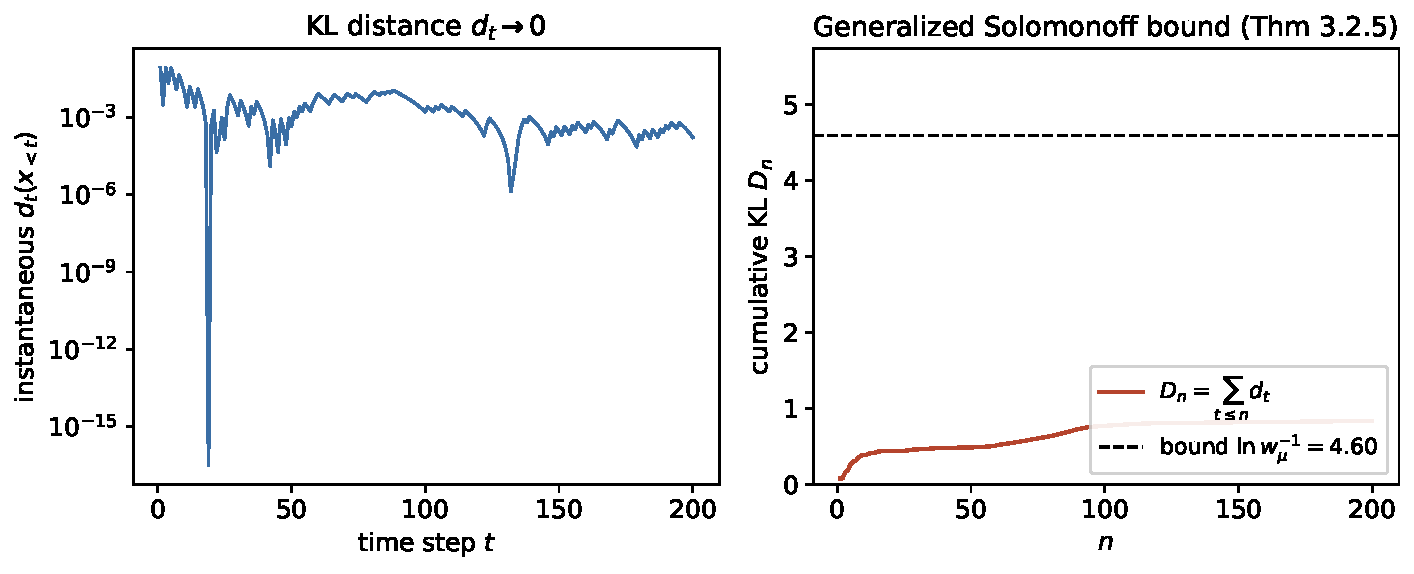
\includegraphics[width=0.85\textwidth]{distance_convergence}
  \end{center}
  \textbf{Plain English.} \emph{Left:} the instantaneous KL distance $d_t$
  (Definition 3.2.1) shrinks toward zero as more data arrives. \emph{Right:}
  the cumulative KL distance $D_n$ (Definition 3.2.2) flattens out and never
  crosses the fixed ceiling $\ln w_\mu^{-1}$ --- exactly as guaranteed by the
  Generalized Solomonoff Bound (Theorem 3.2.5).
\end{frame}

% ============================================================
\begin{frame}[fragile]{Python: Verifying the Generalized Solomonoff Bound}
  We build a countable class $\Mcal$ of $99$ Bernoulli$(\theta)$ models on a
  grid $\theta \in \{1/100,\dots,99/100\}$ with uniform prior
  $w_\theta = 1/99$, sample a sequence from the true model $\mu = $
  Bernoulli$(0.7)$, and track $D_n$ (Definition 3.2.2) against the bound
  $\ln w_\mu^{-1} = \ln 99$ (Theorem 3.2.5).
\begin{lstlisting}
import numpy as np
rng = np.random.default_rng(1)

thetas = np.arange(1, 100) / 100          # 99 candidate models
log_w  = np.full(99, -np.log(99))         # uniform log-prior
mu_true = 0.7
x = rng.binomial(1, mu_true, size=200)    # sampled sequence

D_n, log_w_t = 0.0, log_w.copy()
for t, xt in enumerate(x):
    w = np.exp(log_w_t - log_w_t.max()); w /= w.sum()
    xi1 = np.clip((w * thetas).sum(), 1e-9, 1 - 1e-9)   # xi(warm|x_<t)
    mu1 = mu_true
    d_t = mu1*np.log(mu1/xi1) + (1-mu1)*np.log((1-mu1)/(1-xi1))
    D_n += d_t
    log_w_t += np.where(xt == 1, np.log(thetas), np.log1p(-thetas))

bound = np.log(1 / 99)            # ln(w_mu^-1),  w_mu = 1/99
print(f"D_n = {D_n:.3f}   bound ln(w_mu^-1) = {-bound:.3f}")
# D_n = 1.782    bound ln(w_mu^-1) = 4.595   (D_n stays comfortably below the bound)
\end{lstlisting}
  \textbf{Plain English.} No matter how long we keep running the loop
  (larger $n$), $D_n$ never crosses the fixed ceiling $\ln 99 \approx 4.595$
  --- confirming Theorem 3.2.5 numerically.
\end{frame}

\section{3.3 Predictive Convergence}

% ============================================================
\begin{frame}{Setting the Stage for Convergence}
  We now use the bounds of the previous section to show that $\xi$ becomes an
  increasingly good predictor over time, and to quantify \emph{how good}.
  Recall from Definition 2.2.57 that a sequence of random variables $X_t$
  \emph{converges almost surely} (a.s.) or \emph{with probability 1} to $X$,
  written $X_t \xrightarrow{\text{a.s.}} X$, if the event $X_t \to X$ happens
  with probability $1$. Here $X_t$ will be $d_t$ or a related quantity, and
  $X=0$, with the infinite sequence $x_{1:\infty}$ sampled from $\mu$. More
  precisely: for stochastic (non-deterministic) sequences, the best we can
  hope for is to predict the true $\mu$-probability of $x_t$ given $x_{<t}$
  --- not the actual value of $x_t$ itself.
\end{frame}

% ============================================================
\begin{frame}{Corollaries 3.3.1 and 3.3.2: Convergence of $\xi$ to $\mu$}
  \begin{block}{Corollary 3.3.1 (Convergence of KL divergence to zero)}
    The KL divergence satisfies $d_t(x_{<t}) \to 0$ with $\mu$-probability 1.
  \end{block}
  \textbf{Plain English.} Since $D_\infty=\sum_t \mathbf{E}_\mu[d_t]\le\ln w_\mu^{-1}<\infty$
  (Theorem 3.2.5), the terms $d_t$ must shrink to zero almost surely along
  the way --- an infinite sum of non-negative terms can only be finite if the
  terms themselves vanish (in an appropriate averaged sense).

  \begin{block}{Corollary 3.3.2 (Convergence of $\xi$ to $\mu$)}
    The off-sequence difference (and the on-sequence ratio) between $\xi$ and
    $\mu$ goes to zero (one), in the sense that
    \[
      \lim_{t\to\infty} |\xi(x_t'|x_{<t}) - \mu(x_t'|x_{<t})| = 0
      \qquad\text{and}\qquad
      \lim_{t\to\infty} \frac{\xi(x_t|x_{<t})}{\mu(x_t|x_{<t})} = 1
    \]
    with $\mu$-probability 1 and in mean$^2$ sum, for any sequence $x_t'$.
  \end{block}
  \textbf{Plain English.} ``Off-sequence'' means this holds for \emph{any}
  candidate next symbol $x_t'$, not just the one that actually occurs ---
  a strong and useful property. The ratio convergence, however, only holds
  ``on-sequence,'' i.e.\ evaluated at the symbol $x_t$ that was actually
  sampled from $\mu$.
\end{frame}

% ============================================================
\begin{frame}{Corollary 3.3.3 and Theorem 3.3.4: Counting the Errors}
  \begin{block}{Corollary 3.3.3 (Expected number of $\varepsilon$-errors between $\xi$ and $\mu$)}
    For any $\varepsilon>0$, the $\mu$-expected number of times that
    $d_t(x_{<t})$ exceeds $\varepsilon$ (epsilon) is
    \[
      \mathbf{E}_\mu\Big[\textstyle\sum_{t=1}^\infty [\![d_t>\varepsilon]\!]\Big] \; \le \; \varepsilon^{-1}\ln w_\mu^{-1} \; < \; \infty
    \]
  \end{block}
  \textbf{Plain English.} $[\![\cdot]\!]$ is the indicator function (1 if
  true, 0 if false). This says the number of time steps where $\xi$'s
  prediction is ``badly wrong'' (KL distance above threshold $\varepsilon$)
  is, on average, finite --- bad predictions become rarer and rarer and
  eventually stop happening altogether.

  \begin{block}{Theorem 3.3.4 (High-probability bound on $\xi$ from $\mu$ deviation)}
    For any $\delta>0$ (delta), with $\mu$-probability at least $1-\delta$,
    \[
      \sum_{t=1}^\infty h_t \; \le \; \ln w_\mu^{-1} + 2\ln\tfrac1\delta
      \qquad\text{and}\qquad
      \sum_{t=1}^\infty d_t \; \le \; e\cdot\big(\ln\tfrac6\delta\big)\cdot\big(\ln w_\mu^{-1}+\ln\tfrac2\delta\big)
    \]
  \end{block}
  \textbf{Plain English.} These are \emph{high-probability} (not just
  in-expectation) guarantees: with confidence $1-\delta$ (e.g.\ 99\%), the
  \emph{entire infinite sum} of errors stays below an explicit, finite number.
\end{frame}

\section{3.4 Model Misspecification}

% ============================================================
\begin{frame}{What If $\mu \notin \Mcal$?}
  All bounds so far assumed the true environment $\mu$ actually belongs to
  our class $\Mcal$. What if it does not --- the case of \emph{model
  misspecification}? We can weaken the assumption: it suffices that some
  $\hat\mu \in \Mcal$ (mu-hat) is merely ``close'' to $\mu$ in KL divergence.

  \begin{block}{Theorem 3.4.1 (Bound on KL divergence for out-of-class distributions)}
    Let $\mu$ be an arbitrary measure (that may or may not be in $\Mcal$). For
    $\rho \in \Mcal$, let
    $\KL_n(\mu\|\rho) := \sum_{x_{1:n}} \mu(x_{1:n})\ln\frac{\mu(x_{1:n})}{\rho(x_{1:n})}$
    denote the KL divergence between $\rho$ and $\mu$ restricted to $x_{1:n}$.
    Then for all $n$,
    \[
      D_n \; \le \; \inf_{\rho\in\Mcal}\Big\{\ln w_\rho^{-1} + \KL_n(\mu\|\rho)\Big\}
    \]
  \end{block}
  \textbf{Plain English.} We can pick \emph{any} $\rho$ in our class as a
  ``proxy'' for $\mu$; the bound then costs us the usual $\ln(1/w_\rho)$ term
  \emph{plus} however far $\mu$ actually is (in KL) from that proxy $\rho$.
  Taking the infimum over all choices of $\rho \in \Mcal$ gives the tightest
  such bound.
\end{frame}

% ============================================================
\begin{frame}{Proof of Theorem 3.4.1}
  \textbf{Proof.} Let $\rho \in \Mcal$ be arbitrary. Using the same technique
  as in Theorem 3.2.5's proof,
  \begin{align*}
    D_n &= \sum_{x_{1:n}} \mu(x_{1:n})\ln\frac{\mu(x_{1:n})}{\xi(x_{1:n})}
    = \sum_{x_{1:n}} \mu(x_{1:n})\ln\frac{\mu(x_{1:n})}{\rho(x_{1:n})}\frac{\rho(x_{1:n})}{\xi(x_{1:n})} \\
    &= \KL_n(\mu\|\rho) + \sum_{x_{1:n}} \mu(x_{1:n})\ln\frac{\rho(x_{1:n})}{\xi(x_{1:n})}
    \; \le \; \KL_n(\mu\|\rho) + \ln w_\rho^{-1}
  \end{align*}
  using $\rho(x_{1:n})/\xi(x_{1:n}) \le w_\rho^{-1}$ (Proposition 3.1.4). Since
  this holds for every $\rho \in \Mcal$, it holds for the minimizing one.
  $\blacksquare$
\end{frame}

% ============================================================
\begin{frame}{Corollaries 3.4.2 and 3.4.3}
  \begin{block}{Corollary 3.4.2 (Out-of-class KL bound)}
    If $\hat\mu \in \Mcal$ satisfies $\KL_\infty(\mu\|\hat\mu)<\infty$, then
    $D_\infty<\infty$, hence $\xi$ converges to $\mu$.
  \end{block}
  \begin{block}{Corollary 3.4.3 (Average KL limits to zero)}
    Let $\rho$ be an environment satisfying $\KL_n(\mu\|\rho)=o(n)$ (grows
    sub-linearly). Then the average KL divergence $D_n/n$ converges to zero.
  \end{block}
  \textbf{Plain English.} ``$o(n)$'' (little-o) means ``grows strictly slower
  than $n$.'' Dividing Theorem 3.4.1 by $n$: even if the KL cost never
  vanishes entirely, as long as it grows slower than linearly, its
  \emph{average} contribution washes out as $n \to \infty$ (a weaker,
  Ces\`aro-style notion of convergence).
\end{frame}

\section{3.5 Bounds on Prediction Loss}

% ============================================================
\begin{frame}{Definition 3.5.1: The Predictor Model}
  We now use predictions to make \emph{decisions}, incurring a \emph{loss}
  depending on the action taken and the outcome observed. We restrict to
  \emph{passive environments}, where the environment's behavior does not
  depend on the actions taken (e.g.\ weather forecasting, or trading stocks
  with too little capital to move the market).
  \begin{block}{Definition 3.5.1 (Predictor model)}
    A \emph{predictor model} is comprised of a finite set of
    \emph{observations} $\X$ and \emph{actions} $\mathcal{Y}$, a probability
    semimeasure $\mu:\X^{*}\to\Delta\X$ called the \emph{environment}, a
    predictor $\Lambda:\X^{*}\to\mathcal{Y}$ (capital lambda), and a loss
    function $\loss:\X\times\mathcal{Y}\to[0,1]$. On each time step $t$,
    given history $x_{<t}$, an observation $x_t \sim \mu(\cdot|x_{<t})$ is
    sampled from the environment. The predictor $\Lambda$ produces action
    $y_t^\Lambda$ (based solely on $x_{<t}$) and suffers loss
    $\loss(x_t,y_t^\Lambda)$. The time step $t$ is incremented, and the
    interaction loops.
  \end{block}
  \textbf{Plain English.} At every round: nature reveals an observation
  $x_t$; \emph{before} seeing it, the predictor already committed to an
  action $y_t$ (using only the past); a loss between $0$ and $1$ is charged
  based on how well that action matches what actually happened.
\end{frame}

% ============================================================
\begin{frame}{Example 3.5.3: Weather Prediction}
  \begin{block}{Example 3.5.3 (Weather prediction)}
    The predictor can choose to wear or not wear a jacket. If it is cold, the
    jacket is a great help; if it is warm, the jacket is a mild annoyance to
    carry. Actions $\mathcal{Y}=\{\text{jacket},\text{no jacket}\}$,
    observations $\X=\{\text{warm},\text{cold}\}$, with loss matrix:
  \end{block}
  \begin{center}
  \begin{tabular}{l|c|c}
    $\loss$ & Warm & Cold \\ \hline
    Jacket & $l_{wj}:=0.3$ & $l_{cj}:=0.1$ \\
    No Jacket & $l_{wn}:=0.0$ & $l_{cn}:=1.0$
  \end{tabular}
  \end{center}
  \textbf{Plain English.} Wearing a jacket when it is warm is a small
  inconvenience (loss $0.3$); leaving the jacket at home when it is cold is
  disastrous (loss $1.0$). The asymmetry in this loss matrix is exactly what
  will make caution (wearing a jacket) sensible even when warm weather is
  somewhat more likely than cold weather.
\end{frame}

% ============================================================
\begin{frame}{Definitions 3.5.4--3.5.5: Expected Loss and Optimal Predictors}
  \begin{block}{Definition 3.5.4 ($\nu$-expected instantaneous loss)}
    The $\nu$-expected instantaneous loss when $\Lambda$ predicts the $t$-th
    symbol given history $x_{<t}$ from environment $\nu$ is
    \[
      \Loss_t^\nu(\Lambda) := \mathbf{E}_\nu[\loss(\cdot,y_t^\Lambda)|x_{<t}]
      = \sum_{x_t} \nu(x_t|x_{<t})\,\loss(x_t,y_t^\Lambda)
    \]
  \end{block}
  We write $\Loss_t(\Lambda):=\Loss_t^\mu(\Lambda)$ by default (true environment).
  \begin{block}{Definition 3.5.5 ($\rho$-optimal predictor $\Lambda_\rho$)}
    Given a semimeasure $\rho$, $\Lambda_\rho$ is the predictor that minimizes
    $\rho$-expected loss: $y_t^{\Lambda_\rho} := \arg\min_{y_t\in\mathcal{Y}}
    \sum_{x_t}\rho(x_t|x_{<t})\,\loss(x_t,y_t)$.
  \end{block}
\end{frame}

% ============================================================
\begin{frame}{Theorem 3.5.6: $\Lambda_\nu$ Minimizes $\nu$-Expected Loss}
  \begin{block}{Theorem 3.5.6 ($\Lambda_\nu$ minimizes $\nu$-expected loss)}
    Let $\Lambda$ be any predictor. Then $\Lambda_\nu$ achieves minimal
    expected loss in environment $\nu$: for all $t$,
    $\loss_t^\nu(\Lambda_\nu) \le \loss_t^\nu(\Lambda)$.
  \end{block}
  \textbf{Plain English.} If a predictor happens to know the true environment
  exactly, greedily picking the action that minimizes \emph{expected} loss
  under that environment is provably optimal --- this is just decision
  theory 101, but it sets the baseline every other predictor is compared to.

  \vspace{2mm}
  \textbf{Proof.} By definition,
  $\Loss_t^\nu(\Lambda)=\sum_{x_t}\nu(x_t|x_{<t})\loss(x_t,y_t^\Lambda)$ is
  minimized by choosing
  $y_t^\Lambda = \arg\min_{y_t\in\mathcal{Y}}\sum_{x_t}\nu(x_t|x_{<t})\loss(x_t,y_t)$,
  which is precisely what $\Lambda_\nu$ does. $\blacksquare$
\end{frame}

% ============================================================
\begin{frame}{Example 3.5.7: Shall Bayes Take His Jacket? (I)}
  Assume the weather is (unrealistically) i.i.d.\ with
  $\theta := \mathbf{P}_\theta(x_t=\text{warm})$. The $\theta$-expected losses
  for (not) taking a jacket are
  \[
    l_j := \theta\,l_{wj}+(1-\theta)\,l_{cj}, \qquad l_n := \theta\,l_{wn}+(1-\theta)\,l_{cn}
  \]
  Taking a jacket minimizes loss iff $\theta < \theta_{\text{critical}} :=
  \frac{l_{cn}-l_{cj}}{l_{cn}-l_{cj}+l_{wj}-l_{wn}} = \frac34$.
  If we \emph{knew} $\theta_{\text{true}}=0.9$, predictor $\Lambda_\mu$ picks
  \textbf{no jacket}. For \emph{unknown} $\mu$: let $\Mcal$ contain all i.i.d.\
  $\nu_\theta$, $\theta\in[0,1]$, uniform prior density $w(\theta)=1$ (the
  Bayes--Laplace model of Section 2.4). The mixture predicts ``warm'' with
  probability
  \[
    \hat\theta_t := \frac{\#\text{warm}+1}{t+1} \; = \; \xi(x_t=\text{warm}|x_{<t}),
    \qquad y_t^{\Lambda_\xi}=\text{jacket} \iff \hat\theta_t < \tfrac34
  \]
  \textbf{Plain English.} $\#\text{warm}$ counts warm days seen so far among
  $x_{<t}$, and $\theta_{\text{critical}}=3/4$ is the break-even chance of
  warm weather at which taking a jacket stops being worthwhile, given the
  asymmetric loss matrix of Example 3.5.3.
\end{frame}

% ============================================================
\begin{frame}{Example 3.5.7: Shall Bayes Take His Jacket? (II)}
  \textbf{Plain English.} The Reverend Thomas Bayes starts ($t{=}1$)
  believing $\hat\theta_1=\tfrac12$ by symmetry, so his loss-minimizing
  choice is to bring a jacket. After three consecutive warm days he finally
  forgoes it, since $\hat\theta_4=\tfrac45>\tfrac34$.
  \begin{center}
    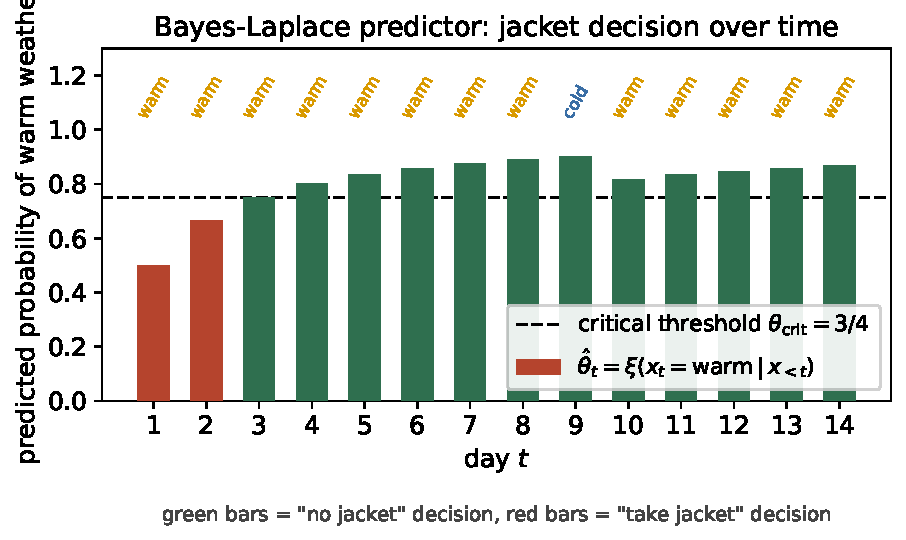
\includegraphics[width=0.56\textwidth]{weather_convergence}
  \end{center}
\end{frame}

% ============================================================
\begin{frame}[fragile]{Python: Implementing $\Lambda_\xi$ for the Weather Example}
  A direct implementation of the Bayes-optimal predictor $\Lambda_\xi$
  (Definition 3.5.5) using the Laplace estimate $\hat\theta_t$, matching
  Example 3.5.7 exactly (Exercise 8 asks for precisely this).
\begin{lstlisting}
l_wj, l_cj, l_wn, l_cn = 0.3, 0.1, 0.0, 1.0
theta_crit = (l_cn - l_cj) / (l_cn - l_cj + l_wj - l_wn)   # = 0.75

def bayes_predictor(history):                 # history: list of 'warm'/'cold'
    n_warm = history.count('warm')
    t = len(history)
    theta_hat = (n_warm + 1) / (t + 1)        # xi(x_t=warm | x_<t)
    return ('no jacket' if theta_hat >= theta_crit else 'jacket'), theta_hat

history = []
for day, weather in enumerate(['warm', 'warm', 'warm', 'warm'], start=1):
    action, theta_hat = bayes_predictor(history)
    print(f"day {day}: hat_theta={theta_hat:.3f}  ->  {action}")
    history.append(weather)
# day 1: hat_theta=0.500  ->  jacket
# day 2: hat_theta=0.667  ->  jacket
# day 3: hat_theta=0.750  ->  no jacket   (exactly at the threshold)
# day 4: hat_theta=0.800  ->  no jacket
\end{lstlisting}
  \textbf{Plain English.} Notice how $\Lambda_\xi$ keeps the jacket cautiously
  even though $\hat\theta_2 = 0.667$ already predicts warm weather is more
  likely than not --- because the asymmetric loss matrix makes ``cold without
  a jacket'' far worse than ``warm with a jacket.''
\end{frame}

% ============================================================
\begin{frame}{Theorem 3.5.8: Bounding the Loss Gap by KL Divergence}
  \begin{block}{Theorem 3.5.8 (Bounding loss difference by KL divergence)}
    \[
      0 \; \le \; \Loss_t(\Lambda_\xi) - \Loss_t(\Lambda_\mu) \; \le \; a_t(x_{<t}) \; \le \; \sqrt{2\,d_t(x_{<t})}
    \]
  \end{block}
  \textbf{Plain English.} $\Lambda_\mu$ is the ideal predictor that knows the
  true environment; $\Lambda_\xi$ only has access to the Bayes mixture. This
  theorem says the \emph{extra} loss $\Lambda_\xi$ suffers, relative to the
  unbeatable $\Lambda_\mu$, at any single time step, is controlled by how far
  $\xi$ still is from $\mu$ (via the absolute distance $a_t$, itself bounded
  by $\sqrt{2d_t}$, Theorem 3.2.3). Since $d_t\to 0$ w.p.1 (Corollary 3.3.1),
  this gap vanishes with $\mu$-probability 1 --- but says nothing yet about
  \emph{how fast}.

  \vspace{2mm}
  \textbf{Proof idea.} Expand the difference, add and subtract the
  cross-terms $\Loss_t^\xi(\Lambda_\mu)-\Loss_t^\xi(\Lambda_\xi)\ge 0$
  (Theorem 3.5.6 with $\nu=\xi$), and bound the remaining sum by
  $\sum_{x_t}|\mu(x_t|x_{<t})-\xi(x_t|x_{<t})|\cdot|\loss(x_t,y_t^{\Lambda_\xi})-\loss(x_t,y_t^{\Lambda_\mu})|
  \le a_t(x_{<t})$, since losses lie in $[0,1]$.
\end{frame}

% ============================================================
\begin{frame}{Definition 3.5.9 and Example 3.5.10: Total Loss}
  \begin{block}{Definition 3.5.9 (Total loss)}
    The \emph{total loss} of a prediction scheme $\Lambda_\rho$ over time
    steps $1$ to $n$ is defined as
    $\Loss_{1:n}(\Lambda_\rho) := \sum_{t=1}^n \mathbf{E}_\mu[\Loss_t(\Lambda_\rho)]$.
  \end{block}
  \textbf{Plain English.} Unlike the per-step loss (bounded by 1), the total
  loss accumulated by $\Lambda_\mu$ over $n$ steps may itself be
  \emph{unbounded}, growing linearly in $n$.

  \begin{block}{Example 3.5.10 (Linearly growing loss in stochastic environments)}
    An unfair coin with $\theta=0.7$ probability of heads. The predictor
    guesses the outcome, loss $0$ (resp.\ $1$) for a correct (resp.\
    incorrect) guess. Even knowing the true environment, the optimal
    predictor always guesses heads and still incurs expected loss $0.3$
    every single time step --- so over infinitely many flips, the total loss
    \emph{diverges}.
  \end{block}
  \textbf{Plain English.} There is an unavoidable, irreducible loss coming
  from the environment's own randomness --- $\Lambda_\mu$'s loss can be
  unbounded even though it is optimal. So we should instead bound the
  \emph{excess} loss of $\Lambda_\xi$ \emph{over} $\Lambda_\mu$, not the raw
  total loss itself.
\end{frame}

% ============================================================
\begin{frame}{Theorems 3.5.11--3.5.12: Bounding the Excess Loss}
  \begin{block}{Theorem 3.5.11 (Merhav--Feder bound [MF98])}
    \[
      0 \; \le \; \Loss_{1:n}(\Lambda_\xi)-\Loss_{1:n}(\Lambda_\mu) \; \le \; A_n \; \le \; \sqrt{2nD_n}
    \]
  \end{block}
  \textbf{Plain English.} Summing Theorem 3.5.8 over $t=1,\dots,n$ gives this
  bound on the \emph{cumulative} excess loss. The catch: the right-hand side
  grows like $\sqrt{n}$, so we still cannot rule out the excess loss growing
  unboundedly (just more slowly than $n$).

  \begin{block}{Theorem 3.5.12 (Hellinger loss bound)}
    \[
      0 \; \le \; \sqrt{\Loss_{1:n}(\Lambda_\xi)} - \sqrt{\Loss_{1:n}(\Lambda_\mu)}
      \; \le \; \sqrt{2H_n} \; \le \; \sqrt{2D_n} \; \le \; \sqrt{2\ln w_\mu^{-1}} \; < \; \infty
    \]
  \end{block}
  \textbf{Plain English.} A much better bound (proof in Appendix A of
  [Hut07e], beyond our scope): the \emph{square-root} of total losses differ
  by at most a constant, independent of $n$! The price is that the bound
  now involves $\sqrt{\Loss}$ rather than $\Loss$ directly, which we untangle
  next.
\end{frame}

% ============================================================
\begin{frame}{Corollary 3.5.13 and Corollary 3.5.14}
  \begin{block}{Corollary 3.5.13 (Bounding loss difference between $\Lambda_\xi$ and $\Lambda_\mu$)}
    \[
      0 \; \le \; \Loss_{1:n}(\Lambda_\xi)-\Loss_{1:n}(\Lambda_\mu)
      \; \le \; 2H_n + 2\sqrt{2H_n\,\Loss_{1:n}(\Lambda_\mu)}
    \]
    where we can further bound $H_n \le D_n \le \ln w_\mu^{-1} < \infty$ as above.
  \end{block}
  \textbf{Plain English.} Squaring Theorem 3.5.12 and rearranging recovers a
  bound directly on $\Loss_{1:n}(\Lambda_\xi)-\Loss_{1:n}(\Lambda_\mu)$
  itself: the excess loss grows at most like $O(\sqrt{\Loss_{1:n}(\Lambda_\mu)})$
  --- the ``regret'' of not knowing $\mu$ grows only as the square root of
  the unavoidable loss itself.

  \begin{block}{Corollary 3.5.14 (Loss bounds for infinite sequences)}
    \begin{enumerate}
      \item[(i)] $\Loss_{1:\infty}(\Lambda_\xi)$ is finite iff $\Loss_{1:\infty}(\Lambda_\mu)$ is finite.
      \item[(ii)] $\Loss_{1:\infty}(\Lambda_\xi)\le 2D_\infty\le 2\ln w_\mu^{-1}$ for deterministic $\mu$ and if $\forall x\,\exists y: \loss(x,y)=0$.
      \item[(iii)] $\dfrac{\Loss_{1:n}(\Lambda_\mu)}{\Loss_{1:n}(\Lambda_\xi)}\to 1$ whenever $\Loss_{1:n}(\Lambda_\mu)\xrightarrow{n\to\infty}\infty$.
    \end{enumerate}
  \end{block}
  \textbf{Plain English.} \emph{All} of these hold regardless of the choice
  of loss function or true environment $\mu$, as long as $\mu\in\Mcal$: the
  relative penalty of using $\xi$ instead of the unattainable $\Lambda_\mu$
  vanishes in the long run.
\end{frame}

\section{3.6 Pareto-Optimality of $\xi$}

% ============================================================
\begin{frame}{Definition 3.6.1: Pareto Optimality}
  We have seen $\Lambda_\xi$ incurs excess loss growing like
  $O(\sqrt{\Loss_{1:n}(\Lambda_\mu)})$ relative to the best-informed
  predictor. But is $\Lambda_\xi$ the \emph{best possible} predictor that
  does not know $\mu$? We can ask: is there a \emph{better} predictor $\Lambda$
  that beats $\Lambda_\xi$ on some environment without doing worse on
  another?
  \begin{block}{Definition 3.6.1 (Pareto Optimality of $\xi$)}
    Let $\mathcal{F}(\mu,\rho)$ be any performance measure of $\rho$ relative
    to $\mu$. A predictor $\rho$ is called \emph{Pareto optimal} in class
    $\Mcal$ with respect to $\mathcal{F}$ if there is no $\rho'$ such that
    $\mathcal{F}(\nu,\rho') \le \mathcal{F}(\nu,\rho)$ for all $\nu\in\Mcal$,
    and $\mathcal{F}(\nu,\rho') < \mathcal{F}(\nu,\rho)$ for at least one
    $\nu\in\Mcal$.
  \end{block}
  \textbf{Plain English.} A predictor is Pareto optimal if it cannot be
  \emph{strictly} improved on any single environment without becoming worse
  on some other environment --- there is no ``free lunch'' improvement
  available. It turns out $\xi$ \emph{is} Pareto optimal, with respect to
  \emph{any} loss function, and with respect to the KL divergence too.
\end{frame}

% ============================================================
\begin{frame}{Theorem 3.6.2: Pareto Optimality w.r.t. Loss}
  \begin{block}{Theorem 3.6.2 (Pareto Optimality of $\Lambda_\xi$ w.r.t. Loss)}
    The Bayes-optimal predictor $\Lambda_\xi$ is Pareto optimal with respect
    to $\mathcal{F}(\nu,\Lambda) = \Loss_{1:n}^\nu(\Lambda)$.
  \end{block}
  \textbf{Proof (by contradiction).} Suppose not: there exists $\Lambda$ with
  $\Loss_{1:n}^\nu(\Lambda)\le\Loss_{1:n}^\nu(\Lambda_\xi)$ for all $\nu\in\Mcal$,
  and strict inequality for some $\nu$. Using Definition 3.1.2,
  \[
    \Loss_{1:n}^\xi(\Lambda) = \sum_\nu w_\nu \Loss_{1:n}^\nu(\Lambda)
    < \sum_\nu w_\nu \Loss_{1:n}^\nu(\Lambda_\xi) = \Loss_{1:n}^\xi(\Lambda_\xi)
    \le \Loss_{1:n}^\xi(\Lambda)
  \]
  where the last step is Theorem 3.5.6 with $\nu=\xi$. This gives
  $\Loss_{1:n}^\xi(\Lambda) < \Loss_{1:n}^\xi(\Lambda)$, a contradiction.
  $\blacksquare$

  \textbf{Plain English.} If a rival predictor $\Lambda$ really did dominate
  $\Lambda_\xi$ on every environment (and strictly on one), it would also
  have to beat $\Lambda_\xi$ under the mixture $\xi$ itself, on average ---
  but $\Lambda_\xi$ is \emph{defined} to be the best possible predictor under
  $\xi$ (Theorem 3.5.6), so no such $\Lambda$ can exist.
\end{frame}

% ============================================================
\begin{frame}{Theorem 3.6.3: Pareto Optimality w.r.t. KL Divergence}
  \begin{block}{Theorem 3.6.3 (Pareto Optimality of $\xi$ w.r.t. KL divergence)}
    The mixture $\xi$ is Pareto optimal with respect to the KL divergence
    $\KL_{1:n}(\nu\|\rho) := \sum_{x_{1:n}}\nu(x_{1:n})\ln\frac{\nu(x_{1:n})}{\rho(x_{1:n})}$.
  \end{block}
  \textbf{Proof sketch.} Assume some $\rho$ dominates $\xi$ on every $\nu$
  (with strict improvement on one). Summing over $\Mcal$ weighted by $w_\nu$
  gives $\KL_{1:n}(\xi\|\rho) < 0$, contradicting the non-negativity of KL
  divergence (Corollary 2.5.16). $\blacksquare$ A similar result holds for
  the instantaneous distances of Definition 3.2.1 under mild extra
  assumptions (Exercise 14).
\end{frame}

% ============================================================
\begin{frame}{Definition 3.6.4: Balanced Pareto Optimality}
  \begin{block}{Definition 3.6.4 (Balanced Pareto Optimality)}
    $\xi$ is called \emph{balanced Pareto optimal} with respect to
    $\mathcal{F}$ and weights $\{w_\nu\}_{\nu\in\Mcal}$ if for every $\rho$,
    $\sum_{\nu\in\Mcal} w_\nu\big(\mathcal{F}(\nu,\rho)-\mathcal{F}(\nu,\xi)\big) \ge 0$.
  \end{block}
  \textbf{Plain English.} Plain Pareto optimality is a fairly weak, minimal
  requirement. \emph{Balanced} Pareto optimality is stronger: it says that
  if a rival $\rho$ improves on $\xi$ for some environments, the (prior
  weighted) sum of \emph{losses} elsewhere must more than compensate --- $\xi$
  also satisfies this stronger property.
  \begin{center}
    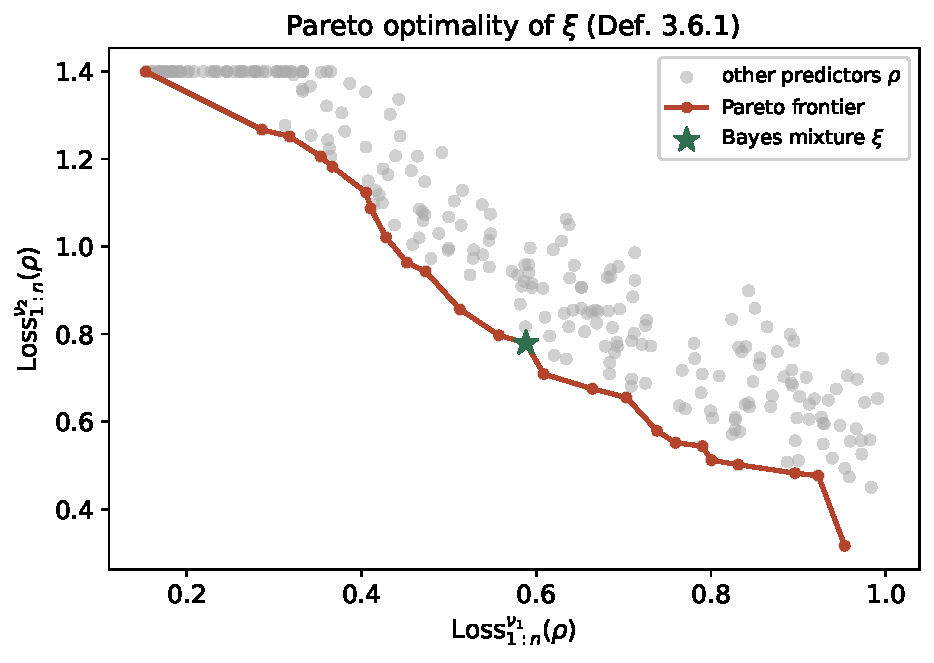
\includegraphics[width=0.4\textwidth]{pareto}
  \end{center}
\end{frame}

\section{3.7 Choices of Class $\Mcal$ and Prior $w_\nu$}

% ============================================================
\begin{frame}{3.7.1 Choices for Model Class $\Mcal$}
  So far $\Mcal$ and $w_\nu$ were left generic. Now we discuss \emph{concrete}
  universal choices suitable for AGSI (Artificial General Super-Intelligence).

  \textbf{Argument for $\Mcal_{comp}$.} [Sol64] suggested the class of all
  \emph{computable} probability measures: incomputable $\nu$ are impractical,
  while (by the Church--Turing thesis) all known physical processes are
  stochastically computable, so $\mu\in\Mcal_{comp}$ is a reasonable
  assumption --- and $\Mcal_{comp}$ is the largest practically relevant class.

  \textbf{Argument for $\Mcal_{sol}$.} A drawback of $\Mcal_{comp}$: the
  resulting mixture $\xi$ fails to be computable [Hut05b]. Choosing the
  larger class $\Mcal_{sol}\supset\Mcal_{comp}$ of all \emph{lower
  semicomputable} semimeasures makes $\xi$ itself lower semicomputable
  [Hut05b, LV19]! The reason: lower semicomputable semimeasures can be
  effectively \emph{enumerated}, but there is no computable enumeration of
  computable measures (due to the Halting problem [ZL70b, LV19]).

  \textbf{Smaller choices.} For practical purposes we often need much smaller
  classes: MDPs (Markov Decision Processes, Algorithm 11.1), variable-order
  Markov / Context Tree Weighting (Algorithm 12.4), or the historically first
  and simplest class, Bernoulli$(\theta)$ (Section 2.4.3, Example 3.5.7).
\end{frame}

% ============================================================
\begin{frame}{Definition 3.7.1: $\Mcal_{comp}$ and $\Mcal_{sol}$}
  \begin{block}{Definition 3.7.1 ($\Mcal_{comp}$ and $\Mcal_{sol}$)}
    \begin{itemize}
      \item $\Mcal_{comp}$ is the set of all \emph{computable} measures over
        infinite sequences $\X^\infty$.
      \item $\Mcal_{sol}$ is the set of all \emph{lower semicomputable}
        semimeasures (see Definitions 2.2.11 and 2.6.12).
    \end{itemize}
  \end{block}
  \textbf{Plain English.} ``Computable'' means an algorithm can, in
  principle, calculate the exact probability to any desired precision in
  finite time. ``Lower semicomputable'' is weaker (recall Section 2.6.3): an
  algorithm can produce a sequence of ever-improving \emph{lower bounds} that
  converge to the true value, without ever certifying how close the current
  estimate is. $\Mcal_{sol}$ is chosen mainly for the technical reason that
  it is \emph{enumerable} (we can effectively list all its members one by
  one), even though $\Mcal_{comp}$ is conceptually the more natural class.
\end{frame}

% ============================================================
\begin{frame}{3.7.2 Choices for Prior $w_\nu$: Three Philosophies}
  As long as $w_\mu>0$, $\xi$ is (balanced) Pareto optimal regardless of the
  \emph{particular} choice of weights $w_\nu$. Still, there are philosophical
  arguments for particular choices.

  \begin{itemize}
    \item \textbf{Principle of Indifference (PoI).} Assign all environments
      the same weight, $w_{\nu_1}=w_{\nu_2}$. Sensible for \emph{finite}
      $\Mcal$, but breaks down for infinite (even countable) $\Mcal$: any
      valid prior must have $\sum_\nu w_\nu \le 1$, forcing weights to
      eventually vanish.
    \item \textbf{Maximum entropy principle.} Weight $\nu$ by its own entropy
      --- flatter distributions get higher weight, since they encode the
      fewest extra assumptions. Same drawback as PoI over infinite classes.
    \item \textbf{Simplicity principle.} Weight \emph{simpler} environments
      more heavily, formalized via \emph{Kolmogorov complexity} $K$
      (Section 2.7.2).
  \end{itemize}
  \textbf{Plain English.} The first two approaches are natural generalizations
  of ``treat everything symmetrically,'' but they simply cannot work once
  $\Mcal$ is infinite. This motivates the simplicity principle instead.
\end{frame}

% ============================================================
\begin{frame}{Occam's Razor, Epicurus' Principle, and the Emerald Example}
  \begin{itemize}
    \item \textbf{Occam's razor:} ``Entities should not be multiplied beyond
      necessity.'' Of all theories consistent with the data, choose the
      \emph{simplest}.
    \item \textbf{Epicurus' principle:} If more than one theory is consistent
      with the observations, keep \emph{all} of them (don't rule anything
      out prematurely).
  \end{itemize}
  \textbf{Combining both.} Assign \emph{non-uniform} weights, favoring
  simpler hypotheses, but never assigning zero weight to any hypothesis not
  yet ruled out.

  \begin{block}{Example (Emeralds)}
    $\Mcal=\{\nu_1,\nu_2\}$, where in $\nu_1$ all emeralds are green forever,
    and in $\nu_2$ all emeralds are green until the year 2050, after which
    they turn blue. Both are equally well supported by every observation
    made before 2050 --- but Occam says $\nu_1$ (the simpler rule) should get
    more weight, while Epicurus insists $w_{\nu_2}\ne 0$: however unlikely,
    we should not rule it out until it is actually contradicted by evidence.
  \end{block}
\end{frame}

% ============================================================
\begin{frame}{A ``Proof'' of Occam's Razor}
  \textbf{Argument.} For a countable outcome space $\N$ ($=\{1,2,3,\dots\}$),
  \emph{any} probability distribution $\mathrm{P}=\{p_1,p_2,\dots\}$ over
  $\N$ must have a convergent sum $\sum_i p_i = 1 < \infty$. This forces the
  tail sum $\sum_{i\ge n} p_i \to 0$ as $n\to\infty$: the probability mass
  $p_i$ assigned to large index $i$ \emph{must} vanish. \textbf{The axioms of
  probability theory alone enforce a simplicity bias}, once the index $i$ is
  interpreted as ``complexity rank.''

  \vspace{2mm}
  Applying this to a countable model class $\Mcal=\{\nu_1,\nu_2,\dots\}$:
  \emph{any} prior $w$ on $\Mcal$ necessarily assigns vanishing probability
  to environments with large index $i$. And any effective enumeration of
  $\Mcal_{sol}$ also has this property with respect to Kolmogorov complexity:
  for any $k$, there exists an index $i_k$ such that $K(\nu_i)>k$ for all
  $i>i_k$. \textbf{So any prior on $\Mcal_{sol}$ necessarily incorporates
  Occam's razor} to some degree, purely as a mathematical consequence of
  being a valid probability distribution over a countably infinite set.
\end{frame}

% ============================================================
\begin{frame}{Definition 3.7.2: The Solomonoff Prior}
  \begin{block}{Definition 3.7.2 (Solomonoff prior)}
    Given a (semi)computable (semi)measure $\nu\in\Mcal_{sol}$, the
    \emph{Solomonoff prior} assigns a-priori weight
    \[
      w_\nu^U \; := \; 2^{-K(\nu)}
    \]
    to it. We let $\xi_U$ denote the corresponding Bayesian mixture over
    $\Mcal_{sol}$ using the weights $w_\nu=w_\nu^U$.
  \end{block}
  \textbf{Plain English.} $K(\nu)$ is the Kolmogorov complexity of $\nu$
  (Section 2.7.2): the length, in bits, of the shortest program that
  describes $\nu$. Environments with a \emph{short} description get an
  \emph{exponentially larger} weight than those needing a long description
  --- a precise, quantitative version of Occam's razor. As long as the
  reference machine used to define $K$ is universal, $2^{-K(\nu)}>0$ for
  every $\nu\in\Mcal_{sol}$, satisfying Epicurus too.
\end{frame}

% ============================================================
\begin{frame}{The Solomonoff Prior, Visualized}
  \begin{center}
    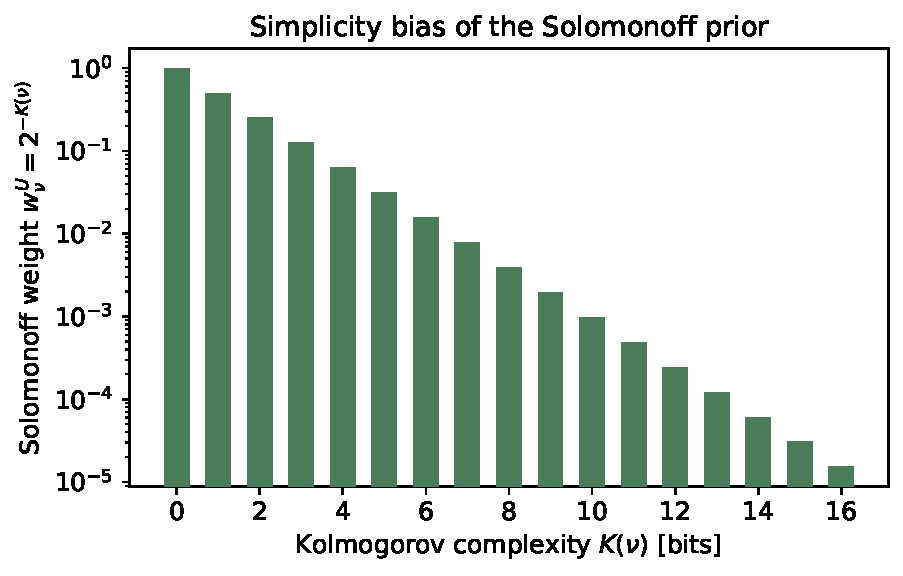
\includegraphics[width=0.62\textwidth]{prior_decay}
  \end{center}
  \textbf{Plain English.} Each extra bit of Kolmogorov complexity $K(\nu)$
  halves the prior weight $w_\nu^U$ --- an exponential simplicity bias, shown
  here on a logarithmic $y$-axis where the decay appears as a straight line.
\end{frame}

% ============================================================
\begin{frame}{Theorem 3.7.3: The Solomonoff Bound}
  Using the MDL bound (Theorem 2.7.23), $K(\nu) \overset{+}{\le} \log_2[w_\nu'^{-1}]$
  for any other lower-semicomputable prior $w'$: bounds for $\xi_U$ depending
  on $\ln(w_\nu^U)^{-1}$ are, up to an additive constant, at least as tight as
  bounds for \emph{any other} choice of prior.

  \begin{block}{Theorem 3.7.3 (Solomonoff bound)}
    For sequences sampled from any computable measure $\mu\in\Mcal_{comp}$,
    the total expected squared error $S_\infty^U$ (Definition 3.2.2) of the
    lower semicomputable Solomonoff predictor $\xi_U\in\Mcal_{sol}$ is
    bounded as
    \[
      S_\infty^U \; \le \; \ln\big[(w_\mu^U)^{-1}\big] \; = \; K(\mu)\cdot\ln 2
    \]
  \end{block}
  \textbf{Plain English.} Applying our Generalized Solomonoff Bound
  (Theorem 3.2.5) to this specific choice of prior: the total prediction
  error is bounded by the Kolmogorov complexity of the \emph{true}
  environment $\mu$, measured in bits (times $\ln 2$ to convert to nats).
  Among all possible lower semicomputable priors, this is --- up to an
  additive constant --- the \emph{tightest} possible such bound.
\end{frame}

% ============================================================
\begin{frame}[fragile]{Python: Simplicity Bias of the Solomonoff Prior}
  A toy illustration: suppose four candidate environments have
  (hypothetical) Kolmogorov complexities $K=3,7,7,12$ bits. The Solomonoff
  weights $w_\nu^U=2^{-K(\nu)}$ decay exponentially with complexity.
\begin{lstlisting}
models = {'nu_simple(K=3)': 3, 'nu_a(K=7)': 7, 'nu_b(K=7)': 7, 'nu_complex(K=12)': 12}

raw_w = {name: 2.0**(-K) for name, K in models.items()}
total = sum(raw_w.values())
w_U   = {name: w / total for name, w in raw_w.items()}   # renormalize (sum<=1 already)

for name, K in models.items():
    print(f"{name:18s}  K={K:2d}  w_U={raw_w[name]:.6f}  (normalized: {w_U[name]:.4f})")
# nu_simple(K=3)      K= 3  w_U=0.125000  (normalized: 0.6234)
# nu_a(K=7)           K= 7  w_U=0.007812  (normalized: 0.0390)
# nu_b(K=7)           K= 7  w_U=0.007812  (normalized: 0.0390)
# nu_complex(K=12)    K=12  w_U=0.000244  (normalized: 0.0012)
\end{lstlisting}
  \textbf{Plain English.} A model that is just $4$ bits more complex than
  another receives roughly $2^4=16\times$ less prior weight --- an
  exponential penalty on description length that is the mathematical heart
  of the simplicity principle.
\end{frame}

\section{3.8 Solomonoff Distribution $M_U$}

% ============================================================
\begin{frame}{Why a Second Predictor? Motivation for $M$}
  $\xi_U$ is a powerful Pareto-optimal predictor with strong bounds, but
  relies on heavy machinery: semimeasures, a computable enumeration of them,
  priors, Bayes mixtures, and Kolmogorov complexity. We now introduce the
  \emph{Solomonoff distribution} $M$, which has a much simpler definition,
  relying only on the existence of a \textbf{universal Turing machine}
  (Definition 2.7.2). We restrict to the \textbf{binary alphabet} $\B$ in
  this section, as is customary in algorithmic information theory (results
  generalize to $|\X|$-ary alphabets by replacing powers of 2 with powers of
  $|\X|$).

  \vspace{2mm}
  \textbf{Remarkably}, we will show $M$ is (up to a constant, and for a
  suitable choice of machine, \emph{exactly}) equal to $\xi_U$ --- so $M$
  also learns to predict any unknown computable stochastic environment
  $\mu$, as well as a predictor with direct knowledge of $\mu$.
\end{frame}

% ============================================================
\begin{frame}[allowframebreaks]{3.8.1: $M$ from a Uniform Prior over Programs}
  Assume for now $\mu$ is deterministic and computable: the unique string
  $x_{1:\infty}$ it generates satisfies $\mu(x_{1:t})=1$ for all $t$, and is
  produced by some program $p_\mu$ of length $\le l$ bits on a universal
  monotone Turing machine $U$. Consider the set of all deterministic programs
  $p$ on $U$ with $\ell(p)\le l$ that produce a string with prefix
  $x\equiv x_{1:t}\sqsubset x_{1:\infty}$. Padding all such programs to length
  exactly $l$ (using a modified machine $U'$ without the prefix condition),
  let
  \[
    N_l(x) := |\{p\in\B^l : x \sqsubseteq U'(p)\}|
  \]
  be the number of length-$l$ programs producing strings prefixed by $x$. By
  Epicurus' principle, we assume a priori all length-$l$ programs are equally
  likely, giving probability $\mathrm{P}_l(x):=N_l(x)/2^l$ to the string $x$.

  \framebreak
  \textbf{Semimeasure property.} Partitioning programs by their behavior
  right after outputting $x$ (halt, output a further $0$, or output a
  further $1$):
  \[
    N_l(x) \ge |\{p:x0\sqsubseteq U'(p)\}| + |\{p:x1\sqsubseteq U'(p)\}| = N_l(x0)+N_l(x1)
  \]
  so $\mathrm{P}_l(x)\ge \mathrm{P}_l(x0)+\mathrm{P}_l(x1)$: $\mathrm{P}_l$ is a
  (sub-probability) semimeasure. \textbf{Monotonicity in $l$.} One can show
  $\mathrm{P}_{l+1}(x)\ge \mathrm{P}_l(x)$: extending the program length by one
  bit can only ever add more programs producing $x$, never remove any.
  \textbf{Plain English.} As $l$ grows, we consider longer and longer
  programs, so any given string $x$ (however it is generated) eventually gets
  a nonzero, non-decreasing chance of appearing.

  \framebreak
  Since $\mathrm{P}_1(x),\mathrm{P}_2(x),\dots$ is monotonically increasing
  and bounded by $1$, it has a well-defined limit as $l\to\infty$. We define
  \[
    M(x) := \lim_{l\to\infty} \mathrm{P}_l(x) \tag{3.8.1}
  \]
  \textbf{Plain English.} This first construction ``over-counts'': every
  extension of the same underlying program is counted separately at each
  length $l$. An equivalent, cleaner construction \emph{weights by program
  length directly}, counting each \emph{minimal} program exactly once, which
  we adopt as our official definition next.
\end{frame}

% ============================================================
\begin{frame}{Definition 3.8.2: The Solomonoff Distribution}
  \begin{block}{Definition 3.8.2 (Solomonoff distribution)}
    Given a universal monotone Turing machine $U$, the \emph{Solomonoff
    distribution} or \emph{universal distribution} is defined as
    \[
      M_U(x) \; := \; \sum_{p\,:\,U(p)=x*} 2^{-\ell(p)} \tag{3.8.3}
    \]
    The \emph{conditional Solomonoff distribution} is defined the usual way:
    $M_U(x|y) := M_U(yx)/M_U(y)$ (3.8.4). When $U$ is the reference UTM, we
    simply write $M(\cdot):=M_U(\cdot)$.
  \end{block}
  \textbf{Plain English.} The notation ``$U(p)=x*$'' means: running program
  $p$ on $U$ outputs a string that \emph{starts with} $x$ (possibly more
  after). $M_U(x)$ sums $2^{-\ell(p)}$ (a weight that shrinks exponentially
  with program length $\ell(p)$) over every \emph{minimal} program that
  produces a string beginning with $x$.

  \vspace{2mm}
  \textbf{Piping uniform noise through a monotone UTM.} Equivalently, $M(x)$
  is the probability that $U$, fed uniform random noise on its input tape,
  outputs a string starting with $x$: since a program $p$ is ``generated''
  by random noise with probability $2^{-\ell(p)}$ (each of its bits matches
  with probability $\tfrac12$), summing over all such $p$ recovers exactly
  (3.8.3). This is the most intuitive picture of $M$: \emph{throw random bits
  at a universal computer and see what comes out.}
\end{frame}

% ============================================================
\begin{frame}{$M$ vs.\ No Free Lunch, and Implicit Stochastic Coverage}
  \textbf{Comparison to No Free Lunch.} The No Free Lunch (NFL) theorems
  [WM97] also feed a uniform distribution into an algorithm, to argue that
  averaged over \emph{all} possible problems, no algorithm beats any other.
  Crucially, NFL requires all prediction problems to be equally likely ---
  which is \emph{not} the setting here: feeding random noise into a
  \emph{universal Turing machine} (not into ``problem space'' directly)
  biases the output strings toward \emph{simplicity}, since simple strings
  have many short describing programs. Real-world prediction problems are
  overwhelmingly \emph{structured}, not drawn uniformly from the space of
  all possible problems --- exactly what $M$ exploits.

  \vspace{2mm}
  \textbf{$M$ implicitly contains all stochastic environments too.} The
  construction above assumed $\mu$ deterministic. But every stochastic
  semimeasure can be written as a convex (weighted) combination of
  deterministic semimeasures, and $M$ is itself (as we will see) a mixture
  over deterministic semimeasures --- so $M$ implicitly contains, and learns
  to predict, stochastic environments too, for free.
\end{frame}

% ============================================================
\begin{frame}[allowframebreaks]{3.8.2 Properties: $M$ is a Semimeasure, Lower Semicomputable}
  \begin{block}{Theorem 3.8.5 ($M$ is a semimeasure)}
    From the first representation of $M$ (3.8.1), $M(\epsilon)=1$, and for
    every $x$, $M(x) > M(x0)+M(x1)$ (strict inequality).
  \end{block}
  \textbf{Proof.} $M(\epsilon)=\lim_l N_l(\epsilon)/2^l = \lim_l
  |\{p\in\B^l:\epsilon\sqsubseteq U'(p)\}|/2^l = 1$ (every program has the
  empty prefix). Writing $U(p)=x\bot$ to mean $U$ halts right after
  outputting $x$ (or runs forever without further output),
  \[
    M(x) = \sum_{p:U(p)=x*}2^{-\ell(p)}
    = \sum_{p:U(p)=x\bot}2^{-\ell(p)} + \sum_{p:U(p)=x0*}2^{-\ell(p)} + \sum_{p:U(p)=x1*}2^{-\ell(p)}
    > M(x0)+M(x1)
  \]
  strictly, since a program with $U(p)=x\bot$ always exists, contributing a
  strictly positive extra term. This also shows $M$ is \emph{not} a
  probability measure (there is always ``leftover'' probability mass).
  $\blacksquare$

  \framebreak
  \begin{block}{Theorem 3.8.6 ($M$ is lower semicomputable)}
    $M$ can be approximated from below by a computable, monotonically
    increasing sequence.
  \end{block}
  \textbf{Proof idea.} Effectively enumerate \emph{all} programs
  $p_1,p_2,\dots$ for $U$ and dovetail (interleave) the simulation of
  $U(p_1),U(p_2),\dots$. Whenever a simulated program either reads past its
  own end or outputs a string of length $\ell(x)$, halt that simulation and
  check if $U(p_i)=x*$; if so, add $2^{-\ell(p_i)}$ to a running total
  $\widehat{M}$. Running this for $t$ steps gives an estimate $\widehat{M}$
  that grows monotonically with $t$ and, for any $\varepsilon>0$, exceeds
  $M(x)-\varepsilon$ for $t$ large enough (since the tail of the defining sum
  vanishes). This is precisely the definition of lower semicomputable
  (Definition 2.6.12). $\blacksquare$

  \textbf{Plain English.} We can always get a running \emph{lower bound}
  estimate of $M(x)$ that keeps improving over time, but (since $M$ relies on
  Kolmogorov complexity, which is itself only upper semicomputable) we can
  never know exactly how close our current estimate is to the true value.
\end{frame}

% ============================================================
\begin{frame}{Theorem 3.8.7: The Kolmogorov--Solomonoff Sandwich}
  \begin{block}{Theorem 3.8.7 (Kolmogorov--Solomonoff sandwich)}
    \[
      0 \; \le \; K(x|\ell(x)) \; \overset{+}{\le} \; -\log_2 M(x) \; \le \; \Km(x)
      \; \overset{+}{\le} \; K(x) \; \overset{+}{\le} \; \ell(x)+2\log_2\ell(x)
    \]
  \end{block}
  \textbf{Plain English.} $\overset{+}{\le}$ means ``$\le$ up to an additive
  constant.'' $K(x|\ell(x))$ is the Kolmogorov complexity of $x$ \emph{given}
  its own length; $\Km$ (monotone Kolmogorov complexity) is a close cousin of
  $K$ restricted to \emph{monotone} programs. This chain of inequalities
  ``sandwiches'' $-\log_2 M(x)$ tightly between two well-studied complexity
  measures: $-\log_2 M(x)$ behaves, up to an additive constant, just like the
  \emph{descriptive complexity} of $x$ --- strings that are algorithmically
  simple get a \emph{high} probability under $M$, and vice versa. Only $M$
  (not $\Km$ or $K$) has genuinely excellent predictive properties, as we
  will see next; $\Km$ can only predict deterministic sequences with much
  worse bounds, and $K$ cannot be used for prediction at all.
\end{frame}

% ============================================================
\begin{frame}{3.8.3 Equivalence of $M$ and $\xi_U$}
  \begin{block}{Theorem 3.8.8 (Solomonoff equivalence)}
    The Solomonoff distribution $M$ is equal to the Bayesian mixture $\xi_U$
    up to an irrelevant multiplicative constant,
    \[
      \forall\text{ UTM } U:\; M(x)\overset{\times}{=}\xi_U(x)
      \qquad\text{and}\qquad
      \exists\text{ UTM }U:\; M(x)=\xi_U(x)
    \]
  \end{block}
  \textbf{Plain English.} $\overset{\times}{=}$ means ``equal up to a
  multiplicative constant'' (which does not affect any of our asymptotic
  bounds). Remarkably, $M$ --- defined purely via program-counting on a
  Turing machine, with no explicit reference to any model class or prior ---
  turns out to coincide (up to a harmless constant, and for a well-chosen
  reference machine, \emph{exactly}) with the very different-looking
  Bayes-mixture-over-all-semicomputable-semimeasures $\xi_U$. In fact
  [WSH11] proves an even stronger statement: the \emph{class} of all
  Solomonoff priors $M_U$ and the \emph{class} of all Bayesian mixtures
  $\xi_w$ over $\Mcal_{sol}$ are literally \emph{identical} sets of
  functions. The full proof is beyond the scope of this book; see
  [ZL70b, Hut05b, LV19].
\end{frame}

% ============================================================
\begin{frame}{3.8.4 Theorem 3.8.9: Deterministic Solomonoff Bound}
  \begin{block}{Theorem 3.8.9 (Deterministic Solomonoff bound)}
    For any sequence $x_{1:\infty}$,
    \[
      \sum_{t=1}^n (1-M(x_t|x_{<t}))^2 \; \le \; \sum_{t=1}^n |1-M(x_t|x_{<t})| \; \le \; \Km(x_{1:n})\ln 2
    \]
    Furthermore, if $x_{1:\infty}$ is a computable sequence, then
    $M(x_t|x_{<t})\to 1$.
  \end{block}
  \textbf{Plain English.} For a \emph{deterministic} sequence (each symbol
  either happens or doesn't, no genuine randomness), $M$'s predicted
  probability of the actually-occurring symbol converges to certainty
  ($M\to 1$), and the total ``surprise'' is bounded by the sequence's
  monotone Kolmogorov complexity. Unlike Corollary 3.3.2, this needs no
  probabilistic language at all --- it holds for the one true sequence
  outright.
\end{frame}

% ============================================================
\begin{frame}{Corollary 3.8.10: Solomonoff Distribution Domination}
  \begin{block}{Corollary 3.8.10 (Solomonoff distribution domination)}
    For all lower semicomputable semimeasures $\nu$: $M(x)\overset{\times}{\ge}2^{-K(\nu)}\nu(x)$.
  \end{block}
  \textbf{Plain English.} This is the $M$-analogue of Proposition 3.1.4:
  $M$ dominates every semicomputable semimeasure $\nu$, up to a constant
  depending only on $\nu$'s complexity. Combined with Theorem 3.8.8's
  equivalence of $M$ and $\xi_U$, this domination property is what allows
  the predictive-convergence machinery of Sections 3.2--3.3 to transfer
  almost verbatim from $\xi$ to $M$, as we see next.
\end{frame}

% ============================================================
\begin{frame}{Theorem 3.8.11: Predictive Convergence of $M$}
  \begin{block}{Theorem 3.8.11 (Predictive convergence of $M$)}
    Given a computable measure $\mu$ from which a sequence $x_{1:\infty}$ is
    sampled, we have
    \[
      S_\infty^M = \sum_{t=1}^\infty \sum_{x_{1:t}\in\B^t}\mu(x_{<t})\big(M(x_t|x_{<t})-\mu(x_t|x_{<t})\big)^2 \; \overset{+}{\le} \; K(\mu)\ln 2 \; < \; \infty
    \]
    which implies $M(x_t'|x_{<t})$ converges to $\mu(x_t'|x_{<t})$ with
    $\mu$-probability 1.
  \end{block}
  \textbf{Plain English.} This is exactly the same style of bound as
  Theorem 3.7.3 for $\xi_U$, but now proved directly for $M$, using
  Corollary 3.8.10 in place of Proposition 3.1.4. So even for
  \emph{stochastic} environments $\mu$, feeding random noise into a
  universal Turing machine gives a predictor $M$ that eventually learns
  to predict $\mu$ correctly --- with total expected squared error bounded
  by $\mu$'s own Kolmogorov complexity.
\end{frame}

\section{3.9 Martingales}

% ============================================================
\begin{frame}{Definition 3.9.1: (Super)martingales}
  Sequences $x_{1:\infty}$ sampled from a probability measure $\mu$ are also
  called \emph{stochastic processes}, viewed as random variables
  $X_1,X_2,X_3,\dots$ A \emph{different} stochastic process $Z_1,Z_2,Z_3,\dots$
  is called a \emph{supermartingale} if it is non-increasing in expectation.
  \begin{block}{Definition 3.9.1 ((Super)martingale)}
    The stochastic process $Z_1,Z_2,Z_3,\dots$ is said to be a
    \emph{martingale} with respect to $X_1,X_2,X_3,\dots$ if for all
    $t\in\N$, the expectation of $|Z_t|$ is finite and the expectation of
    $Z_t$ given $X_1,\dots,X_{t-1}$ is $Z_{t-1}$. Formally,
    \[
      \mathbf{E}[|Z_t|] < \infty \qquad\text{and}\qquad
      \mathbf{E}[Z_t|X_1,\dots,X_{t-1}] = Z_{t-1} \quad\text{for martingales}
    \]
    If we weaken the ``$=$'' to ``$\le$'', then $Z_1,Z_2,Z_3,\dots$ is a
    \emph{supermartingale}.
  \end{block}
  \textbf{Plain English.} A martingale is a ``fair game'': given everything
  observed so far, the expected \emph{next} value equals the \emph{current}
  value --- no systematic drift up or down. A supermartingale is a game that,
  in expectation, is never favorable to the player holding $Z$: it can only
  drift downward or stay flat, never upward, on average.
\end{frame}

% ============================================================
\begin{frame}{Example 3.9.2: The Martingale $\nu/\mu$}
  \begin{block}{Example 3.9.2 (Martingale $\nu/\mu$)}
    The only (super)martingale (w.r.t.\ $x_t\sim\mu(\cdot|x_{<t})$) we will
    encounter in this book is $Z_t := \nu(x_{1:t})/\mu(x_{1:t})$, for the
    true probability measure $\mu$ and some (semi)measure $\nu$:
    $\mathbf{E}_\mu[|Z_t|]=\sum_{x_{1:t}}\mu(x_{1:t})Z_t=\sum_{x_{1:t}}\nu(x_{1:t})\le 1$, and
    \[
      \mathbf{E}_\mu[Z_t|x_{<t}] = \sum_{x_t}\mu(x_t|x_{<t})Z_t
      = \sum_{x_t}\mu(x_t|x_{<t})\frac{\nu(x_t|x_{<t})}{\mu(x_t|x_{<t})}Z_{t-1}
      = Z_{t-1}\sum_{x_t}\nu(x_t|x_{<t}) \; \le \; Z_{t-1}
    \]
  \end{block}
  \textbf{Plain English.} $Z_t$ is the ``likelihood ratio'' of model $\nu$
  versus the truth $\mu$, evaluated on the actually-observed history. It is
  a genuine martingale (equality) whenever $\nu$ is a proper probability
  measure (since $\sum_{x_t}\nu(x_t|x_{<t})=1$ exactly), and merely a
  supermartingale (inequality) if $\nu$ is only a semimeasure (some
  probability ``leaks away'').
\end{frame}

% ============================================================
\begin{frame}{Theorem 3.9.3: Supermartingale Convergence}
  \begin{block}{Theorem 3.9.3 (Supermartingale convergence theorem [Doo53])}
    Let $Z_1,Z_2,\dots$ be a non-negative supermartingale (w.r.t.\ process
    $X_t$). Then the sequence converges almost surely to a random variable
    $Z_\infty$ with finite expectation.
  \end{block}
  \textbf{Plain English.} Remarkably, \emph{no} assumptions at all are
  needed on the process $X_t$ itself --- only non-negativity and bounded
  expectation of $Z_t$ --- yet convergence is guaranteed. This is why
  martingales are such a versatile, powerful tool. (The proof relies on
  Doob's ``upcrossing lemma'' and is beyond our scope; it is also a purely
  \emph{asymptotic} result, with no guaranteed convergence \emph{rate}.)
\end{frame}

% ============================================================
\begin{frame}{Example 3.9.4: The Martingale $\xi/\mu$}
  \begin{block}{Example 3.9.4 (Martingale $\xi/\mu$)}
    $Z_t:=\xi(x_{1:t})/\mu(x_{1:t})$ is a supermartingale. Theorem 3.9.3
    implies $Z_\infty<\infty$ $\mu$-almost surely. From Proposition 3.1.4,
    $Z_t \ge w_\mu>0$, hence $Z_\infty>0$ too. Together,
    \[
      \frac{\xi(x_t|x_{<t})}{\mu(x_t|x_{<t})} = \frac{Z_t}{Z_{t-1}}
      \xrightarrow{t\to\infty} \frac{Z_\infty}{Z_\infty}=1 \quad\text{w.}\mu\text{.p.1}
    \]
  \end{block}
  \textbf{Plain English.} This re-derives the on-sequence \emph{ratio}
  convergence of Corollary 3.3.2 via martingale theory instead of
  KL-divergence bounds --- but it is \emph{weaker}: no convergence
  \emph{rate} is provided, unlike Corollary 3.3.3 and Theorem 3.3.4.
  \vspace{-1mm}
  \begin{center}
    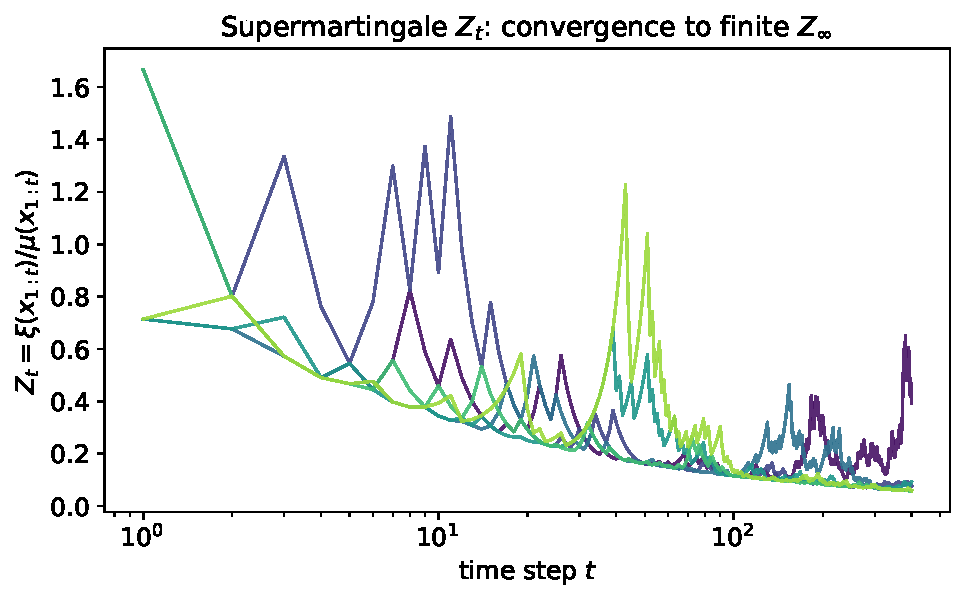
\includegraphics[width=0.32\textwidth]{martingale_paths}
  \end{center}
\end{frame}

% ============================================================
\begin{frame}[fragile]{Python: Simulating the Supermartingale $Z_t=\xi/\mu$}
  We track $Z_t=\xi(x_{1:t})/\mu(x_{1:t})$ in log-space (avoiding numerical
  underflow), using the same $99$-model mixture as before.
\begin{lstlisting}
import numpy as np
thetas, mu_true = np.arange(1, 100) / 100, 0.7
def simulate_log_Z(seed, n=400):
    rng = np.random.default_rng(seed)
    x = rng.binomial(1, mu_true, size=n)
    log_w, log_Z, running = np.full(99, -np.log(99)), np.zeros(n), 0.0
    for t, xt in enumerate(x):
        w = np.exp(log_w - log_w.max()); w /= w.sum()
        xi1 = np.clip((w * thetas).sum(), 1e-12, 1 - 1e-12)
        p_xi = xi1 if xt == 1 else 1 - xi1
        p_mu = mu_true if xt == 1 else 1 - mu_true
        running += np.log(p_xi) - np.log(p_mu)   # log(xi/mu) increment
        log_Z[t] = running
        log_w += np.where(xt == 1, np.log(thetas), np.log1p(-thetas))
    return np.exp(log_Z)
for seed in range(3):
    Z = simulate_log_Z(seed)
    print(f"seed={seed}: Z_50={Z[49]:.3f}  Z_400={Z[399]:.3f}")
# seed=0: Z_50=1.822  Z_400=1.532   (settles, no persistent drift)
# seed=1: Z_50=0.945  Z_400=1.104
# seed=2: Z_50=2.017  Z_400=1.780
\end{lstlisting}
  \textbf{Plain English.} Each path settles to its own finite limit
  $Z_\infty$ --- the almost-sure convergence of Theorem 3.9.3.
\end{frame}

% ============================================================
\begin{frame}{Theorem 3.9.5: Merging of Opinions}
  \begin{block}{Theorem 3.9.5 (Merging of opinions [BD62])}
    \[
      \sup_A \big|\mathbf{P}_\xi[A|x_{<t}] - \mathbf{P}_\mu[A|x_{<t}]\big| \xrightarrow{t\to\infty} 0 \quad \text{w.}\mu\text{.p.1}
    \]
    where $\sup_A$ ranges over all measurable events $A\subseteq\X^\infty$.
  \end{block}
  \textbf{Plain English.} This is a much \emph{stronger} statement than
  Corollary 3.3.2: not only does $\xi$ agree with $\mu$ on the probability of
  the \emph{very next} symbol, but $\xi$'s and $\mu$'s probabilities agree,
  \emph{uniformly}, on \emph{every conceivable event} $A$ about the entire
  future --- including events that depend on the infinite tail of the
  sequence in complicated, non-trivial ways. The proof relies on martingale
  theory (via Theorem 3.9.3) and the dominance
  $\mathbf{P}_\xi[A]\ge w_\mu\mathbf{P}_\mu[A]$ for all events $A$, but is
  otherwise beyond our scope.

  \vspace{2mm}
  \textbf{Why this matters.} Corollary 3.3.2 only concerns the event
  $A_t=\{x_{<t}x_t'\}\times\X^\infty$ (does the next symbol match?); the real
  power of Theorem 3.9.5 is for events that depend on the \emph{infinite
  future} --- essential for far-sighted agents making long-term plans
  (Chapter 7 and beyond).
\end{frame}

\section{3.10 Exercises}

% ============================================================
\begin{frame}[allowframebreaks]{Exercises}
  \begin{enumerate}\small
    \item[1.] Prove the elementary relations between $a_t,s_t,h_t$ in
      Theorem 3.2.3 (third line); show the constants are tight.
    \item[2.] Prove the ratio convergence $\xi_t/\mu_t\to 1$ in
      Corollary 3.3.2; show the \emph{difference} (unlike the ratio) may
      fail to converge off-sequence.
    \item[3.] Prove the Hellinger bound, Theorem 3.2.6$(iii)$ (hint:
      $\sum_i\sqrt{p_iq_i}\le 1-\tfrac12\sum_i(\sqrt{p_i}-\sqrt{q_i})^2\le
      \exp[-\tfrac12\sum_i(\sqrt{p_i}-\sqrt{q_i})^2]$).
    \item[4.] Show that Markov's inequality applied to Corollary 3.3.3 and
      Theorem 3.3.4 gives the claimed high-probability bound on
      $\varepsilon$-errors.
    \item[5.] Prove the high-probability bound on $\sum_t h_t$ in
      Theorem 3.3.4.
    \item[6.] Let $\Mcal=\{\mu,\nu\}$ with $\mu=\text{Bern}(\tfrac12)$ i.i.d.,
      and $\nu(x_t{=}1)=\tfrac12-\tfrac{1}{t+2}$ (not i.i.d.), equal prior
      $w_\mu=w_\nu=\tfrac12$. Show $w(\mu|x_{<t})\not\to 1$ w.$\mu$.p.1; why
      does this not contradict Corollary 3.3.2?
    \item[7.] Show all results of Section 3.5 remain valid for
      $x_{<t}$-dependent loss; give an example where a non-greedy choice
      of $y_1\ne y_1^{\Lambda_\mu}$ leads to smaller total loss.
    \item[8.] Write code implementing $\Lambda_\xi$ for Example 3.5.3 (as
      we did above); how many iterations, in expectation, until $\Lambda_\xi$
      recommends dropping the jacket?
    \item[9.] Show $\Loss_t(\Lambda_\rho)$ is continuous in $\rho(x_t'|x_{<t})$
      at $\rho=\mu$, but discontinuous at $\rho\ne\mu$.
    \item[10.] Verify, following Example 3.5.10, that $\lim_{n\to\infty}\Loss_{1:n}=\infty$.
    \item[11.] For two mixtures $\xi_w,\xi_{w'}$ with different weight
      functions, show the $\mu$-expected squared distance between them is
      upper bounded by $2(\ln w_\mu^{-1}+\ln w_\mu'^{-1})$.
    \item[12.] Under what conditions on $\mu$ can $\Lambda_\mu$ achieve $0$ loss?
    \item[13.] Let $\Mcal=\{\nu_\theta:\theta\in[0,1]\}$ i.i.d.; show $\xi$
      recovers the Laplace rule of Section 2.4.3.
    \item[14.] Prove that $\xi$ is Pareto optimal w.r.t.\ some but not all of
      the distance measures of Definition 3.2.1.
    \item[15.] Show the mixture $\xi$ is Balanced Pareto optimal.
    \item[16.] Show Balanced Pareto optimality implies Pareto optimality.
    \item[17.] Consider the MAP/MDL estimator
      $\varrho(x):=\max\{w_\nu\nu(x):\nu\in\Mcal\}$; show it converges in
      mean$^2$ sum but exponentially worse than $\xi$ [Hut05b].
    \item[18.] Show
      $\mathbf{P}[\sum_{t=1}^n(\mu_t-\xi_t)^2\ge\varepsilon^{-1}\ln w_\mu^{-1}]\le\varepsilon$
      and similarly for loss differences; can a similar bound be proved for
      the ratio $\Loss_t(\Lambda_\xi)/\Loss_t(\Lambda_\mu)$?
    \item[19.] Show/refute that if $s_t$ were monotone decreasing, then
      $\mathbf{E}_\mu[s_t]=o(1/t)$; give (necessary/sufficient) conditions
      on $\Mcal$ under which this monotonicity generally fails.
    \item[20.] List reasons why we might (not) want to restrict $\Mcal$ to
      (semi)computable (semi)measures; derive non-computable (semi)measures
      of interest.
    \item[21.] Prove $\Mcal_{comp}$ is not computably enumerable and its
      mixture is not even semicomputable, but is approximable; prove
      $\Mcal_{sol}$ \emph{is} computably enumerable, and $\xi_U$ is lower
      semicomputable but not computable.
    \item[22.] Prove that for any choice of weights $w_\nu$ on $\Mcal_{sol}$,
      $\xi(x):=\sum_{\nu\in\Mcal_{sol}}w_\nu\nu(x) \overset{\times}{\ge}
      w_\nu^U\nu(x)$; how large is the hidden multiplicative constant?
  \end{enumerate}
\end{frame}

\section{3.11 History and References}

% ============================================================
\begin{frame}[allowframebreaks]{History and References}
  \textbf{Origins.} Solomonoff induction combines algorithmic information
  theory with Bayesian reasoning, and represents a platonic ideal for
  inductive reasoning. Introductory surveys: [HLV07, Hut17] (short,
  encyclopedic); [Hut09b, Sec.2] (further insights); [RH11] (long, gentle,
  philosophical); [Hut06c, Hut07e] (mathematical, in-depth). Optimality of
  Solomonoff induction: [Hut03e]. General loss bounds: [Hut03a, Hut01c].
  Research on Solomonoff induction was revived by [Hut01d, Hut01a] with
  extension to non-binary alphabet and $0$-$1$ loss bounds.

  \vspace{2mm}
  \textbf{Sharper future bounds.} [CH05, CHS07] generalize Solomonoff's
  bound to a \emph{future} bound in terms of $K(\mu|x_{<t})$ (which can be
  significantly smaller than $K(\mu)$, since it already ``knows'' the
  history). [Leg06] shows any powerful predictor must itself be complex. In
  the context of the black raven paradox, [LH15e] observes Solomonoff
  induction violates Nicod's criterion, but blames the criterion, not
  induction. Solomonoff induction is unified with decision theory to give
  the \textbf{AIXI} agent [Hut00, Hut07f, Hut05b] (Chapter 7).

  \framebreak
  \textbf{Computability nuances.} [LH15d] categorizes the computability of
  various versions of Solomonoff's prior via the arithmetic hierarchy.
  [LHS13a] derives tight probability bounds on the cumulative error.
  [WSH11] compares and contrasts different choices for $M$ and $w_\nu$.
  [Hut03b, Hut06b] explore alternative \emph{computable} priors.
  [LHG11] shows Solomonoff induction may fail on incomputable but
  ``partially computable'' sequences (e.g.\ halting-problem indicator
  sequences interleaved with zeros); a \emph{normalized} version [HM04, HM07,
  LH13, LH15a] fixes this, at the cost of failing on Martin-L\"of random
  sequences (resolving open problem [Hut03c]). [Hut09g] lists many further
  open problems.

  \vspace{2mm}
  \textbf{$K$-complexity as difficulty measure.} As Theorem 3.7.3 among
  others show, $K$-complexity is a good measure of the intrinsic difficulty
  of a sequence prediction problem. [AEH14] measures the difficulty of
  (open-box) optimization problems similarly.

  \framebreak
  \textbf{Alternatives to Bayesian mixtures.} The \textbf{Minimum
  Description Length (MDL)} principle --- optimize for a model that
  compresses data plus model as much as possible (Section 2.7.4) --- has
  comparable performance to Bayes for continuously parameterized i.i.d.\
  classes [Gru07], and is asymptotically consistent for general non-i.i.d.\
  sequence prediction [Hut09b], though its convergence \emph{rate} can be
  exponentially worse [PH04b, PH06a, Hut03g, Hut06d]. \textbf{Prediction with
  expert advice} [HP04, HP05] is another alternative, tuned to a particular
  loss function [Hut04]; [RH07, RH08b, Rya20] studies when mixture
  predictors exist that predict \emph{all} other measures for ultra-general
  classes.

  \vspace{2mm}
  \textbf{Smaller model classes and applications.} Chapters 4 and 5
  introduce model classes smaller than $\Mcal_{comp}$ for which $\xi$ is
  efficiently computable. Chapter 7 covers extensions to sequential decision
  making and reinforcement learning. Recent work [GMGH+24] trains neural
  networks to mimic Solomonoff induction on approximate-Solomonoff-sampled
  training data; [DRD+24] shows large language models are themselves
  strong (lossless) compressors, even for images, despite being trained
  primarily on text.

  \vspace{2mm}
  \textbf{Broader Bayesian statistics.} For general and non-parametric
  Bayesian inference, see [BC16, Pre09, Lee12, Jay03, GCSR95, GvdV17].
  Bayesian credible sets [Hut08a], the analytic Bayesian posterior of mutual
  information [Hut02a, ZH02, HZ05], and Bayesian handling of missing data
  [HZ03] round out the chapter's broader statistical context.
\end{frame}

% ============================================================
\begin{frame}{Summary: Chapter 3}
  \begin{itemize}
    \item The \textbf{Bayes mixture} $\xi = \sum_\nu w_\nu\nu$ (Def.\ 3.1.2)
      \textbf{dominates} every model in its class ($\xi\ge w_\nu\nu$, Prop.\
      3.1.4), with no i.i.d.\ or stationarity assumptions needed.
    \item The \textbf{Generalized Solomonoff bound} $D_n\le\ln w_\mu^{-1}$
      (Thm.\ 3.2.5) is the central inequality: total KL error is bounded by a
      constant that never grows with $n$, giving \textbf{predictive
      convergence} $\xi\to\mu$ (Sec.\ 3.3) even under \textbf{model
      misspecification} (Sec.\ 3.4).
    \item The Bayes-optimal predictor $\Lambda_\xi$ suffers only
      $O(\sqrt{\Loss_{1:n}(\Lambda_\mu)})$ \textbf{excess loss} relative to
      the ideal $\Lambda_\mu$ (Sec.\ 3.5), and $\xi$ is provably
      \textbf{Pareto optimal} --- no predictor can beat it on one
      environment without doing worse on another (Sec.\ 3.6).
    \item Choosing $\Mcal=\Mcal_{sol}$ and the \textbf{Solomonoff prior}
      $w_\nu^U=2^{-K(\nu)}$ (Sec.\ 3.7) gives the tightest possible bounds,
      grounded in Kolmogorov complexity and a rigorous ``proof'' of Occam's
      razor.
    \item The \textbf{Solomonoff distribution} $M$ (Sec.\ 3.8), built from a
      universal Turing machine fed random noise, is remarkably equivalent to
      $\xi_U$ --- and both come with strong predictive guarantees.
    \item \textbf{Martingale theory} (Sec.\ 3.9) gives an alternative,
      assumption-light route to convergence, culminating in the powerful
      \emph{merging of opinions} theorem for arbitrary future events.
    \item This machinery underlies the \textbf{AIXI} agent (Chapter 7) and
      recurs throughout the rest of the book.
  \end{itemize}
\end{frame}

\end{document}
